\documentclass{article}[11pt]
% fancybox prevents the TOC from printing
%\usepackage{fancyhdr, fancybox, tabularx, verbatim, epsfig}
\usepackage{fancyhdr, tabularx, verbatim, epsfig}
\usepackage{amssymb,psboxit}
\usepackage{rotating}
\usepackage[pdftex,
            pdfpagemode=none,
            pdfstartview=FitH]{hyperref}

\hypersetup{
  pdfauthor = {Michael W. Gee, Jonathan J. Hu, Marzio G. Sala, Christopher M. Siefert, Ray S. Tuminaro},
  pdftitle = {ML 5.0 Smoothed Aggregation User's Guide},
  colorlinks= {true},
  citecolor = {blue},
}

\setlength{\oddsidemargin}{0.1\oddsidemargin}
\setlength{\evensidemargin}{0.5\evensidemargin}
\setlength{\topmargin}{0.0\topmargin}
\setlength{\textheight}{1.16\textheight}
\setlength{\textwidth}{1.35\textwidth}
\newcommand{\Aztec}  {{\sc Aztec}}
\newcommand{\Aztecoo}  {{\sc AztecOO}}
\newcommand{\aztecoo}  {{\Aztecoo}}
\newcommand{\epetra}  {{\sc Epetra}}
\newcommand{\epetraext}  {{\sc EpetraExt}}
\newcommand{\ML}     {{\bf ML}}
\newcommand{\trilinos}  {{\sc Trilinos}}
\newcommand{\amesos}  {{\sc Amesos}}
\newcommand{\anasazi}  {{\sc Anasazi}}
\newcommand{\umfpack}  {{\sc Umfpack}}
\newcommand{\superlu}  {{\sc SuperLU}}
\newcommand{\superludist}  {{\sc SuperLU\_dist}}
\newcommand{\mumps}  {{\sc Mumps}}
\newcommand{\klu}  {{\sc Klu}}
\newcommand{\metis}  {{\sc Metis}}
\newcommand{\parmetis}  {{\sc ParMetis}}
\newcommand{\triutils}  {{\sc Triutils}}
\newcommand{\ifpack}  {{\sc Ifpack}}
\newcommand{\parasails}  {{\sc ParaSails}}
\newcommand{\teuchos}  {{\sc Teuchos}}
\newcommand{\newpackage}  {{\sc new\_package}}
\newcommand{\zoltan}  {{\sc Zoltan}}
\newcommand{\nox}  {{\sc NOX}}
\newcommand{\loca}  {{\sc Loca}}
\newcommand{\paraview}  {{\sc ParaView}}
\newcommand{\galeri}  {{\sc Galeri}}
\newcommand{\be}  {\begin{enumerate}}
\newcommand{\ee}  {\end{enumerate}}
% Maxwell abbreviations
\newcommand \Ke {\ensuremath{K^{(e)}}}
\newcommand \Kn {\ensuremath{K^{(n)}}}
\newcommand \Th {\ensuremath{T_h}}
%\newcommand \curlcurl {({\it curl,curl})}
\newcommand \curlcurl {\ensuremath{\nabla\times\nabla\times}}
\newcommand \trilinosWeb {trilinos.sandia.gov}
\newcommand \petsc {PETSc}
\newcommand \mlp {{\tt MultiLevelPreconditioner}}

\newcommand{\comm}[2]{\bigskip
                      \begin{tabular}{|p{4.5in}|}\hline
                      \multicolumn{1}{|c|}{{\bf Comment by #1}}\\ \hline
                      #2\\ \hline
                      \end{tabular}\\
                      \bigskip
                     }
%
% ***********************************************************************
% * 02 July 1993: McCorkle                                              *
% * Define a macro that will lightly print the word `DRAFT' diagonally  *
% * across each page of the document. This macro was obtained from the  *
% * NMSU math department                                                *
% *                                                                     *
% * Usage: \draft                                                       *
% ***********************************************************************
%
\def\optionbox#1#2{\noindent$\hphantom{ii}${\parbox[t]{1.5in}{\it
#1}}{\parbox[t]{4.8in}{#2}} \\[1.1em]}

\def\choicebox#1#2{\noindent$\hphantom{th}$\parbox[t]{3.0in}{\sf
#1}\parbox[t]{3.35in}{#2}\\[0.8em]}

\def\structbox#1#2{\noindent$\hphantom{hix}${\parbox[t]{2.10in}{\it
#1}}{\parbox[t]{3.9in}{#2}} \\[.02cm]}

\def\protobox#1{\vspace{2em}{\flushleft{\bf Prototype}
\hrulefill}\flushleft{\fbox{\parbox[t]{6in}{\vspace{1em}{\sf
#1}\vspace{1em}}}}}


\def\draft{%
\special{!userdict begin /bop-hook{gsave
200 30 translate 65 rotate
/Times-Roman findfont 216 scalefont setfont
0 0 moveto 0.9 setgray (DRAFT) show grestore}def end}
}

\begin{document}
\bibliographystyle{siam}
\setcounter{page}{3}

\large

%\draft                                   % Lightly print `DRAFT' on every
                                         % page of the document

%
%
%\hspace{2.22in}
\begin{center}
SAND2006-2649
%\hfill
%\hspace{2.41in}
Unlimited Release \\
%\hfill
%\begin{center}
Printed Feb 2007
\end{center}

\vspace{0.2in}

\begin{center}
{\Large {\bf ML 5.0 Smoothed Aggregation User's Guide}}
%\footnote{ Sandia is a multiprogram laboratory operated by Sandia Corporation,
%a Lockheed Martin Company, for the United States Department of Energy's
%National Nuclear Security Administration under contract DE-AC04-94AL85000.}}}
%\footnote{ This work was supported by
%        the
%        Applied Mathematical Sciences program, U.S. Department of Energy,
%        Office of Energy Research, and was partially performed at 
%        Sandia National
%        Laboratories, operated for the U.S. Department of Energy under contract
%        No. DE-AC04-94AL85000.} }}

\vspace*{0.8in}
Michael W. Gee $\quad$ and $\quad$
Christopher M. Siefert \\
Computational Math \& Algorithms \\
Sandia National Laboratories\\
Mailstop 1320 \\
P.O.~Box 5800 \\
Albuquerque, NM 87185-1320\\[10pt]
Jonathan J. Hu $\quad$ and $\quad$
Ray S. Tuminaro \\
Computational Math \& Algorithms \\
Sandia National Laboratories\\
Mailstop 9159 \\
P.O.~Box 0969 \\
Livermore, CA 94551-0969\\[10pt]
Marzio G. Sala \\
ETH Z\"urich Computational Laboratory\\
CAB F84\\
ETH Zentrum\\
8092 Z\"urich\\


\vspace*{1in}

\end{center}

\begin{abstract}

\ML\ is a multigrid preconditioning package intended to solve linear
systems of equations $A x = b$ where $A$ is a user supplied $n \times n$
sparse matrix, $b$ is a user supplied vector of length $n$ and $x$ is a
vector of length $n$ to be computed. \ML\ should be used on large sparse
linear systems arising from partial differential equation (PDE)
discretizations.  While technically any linear system can be considered,
\ML\ should be used on linear systems that correspond to things that work
well with multigrid methods (e.g. elliptic PDEs).  \ML\ can be used as a
stand-alone package or to generate preconditioners for a traditional
iterative solver package (e.g. Krylov methods). We have supplied support
for working with the {\sc Aztec 2.1} and {\sc AztecOO} iterative packages
\cite{Aztec}.  However, other solvers can be used by supplying a few
functions.

This document describes one specific algebraic multigrid approach:
smoothed aggregation.  This approach is used within several specialized
multigrid methods: one for the eddy current formulation for Maxwell's
equations, and a multilevel and domain decomposition method for
symmetric and non-symmetric systems of equations (like elliptic
equations, or compressible and incompressible fluid dynamics problems).
Other methods exist within \ML\ but are not described in this document.
Examples are given illustrating the problem definition and exercising
multigrid options.

\end{abstract}

%
\clearpage
\newpage

\vfill
\begin{center}
(page intentionally left blank)
\end{center}
\clearpage
\newpage


\tableofcontents
\newpage
%
%
%%%%%%%%%%%%%%%%%%%%%%%%%%%%%%%%%%%%%%%%%%%%%%%%%%%%%%%%%%
\section{Notational Conventions}
%%%%%%%%%%%%%%%%%%%%%%%%%%%%%%%%%%%%%%%%%%%%%%%%%%%%%%%%%%
%

In this guide, we show typed commands in this font:
\begin{verbatim}
% a_really_long_command
\end{verbatim}
The character \verb!%! indicates any shell prompt\footnote{For
  simplicity, commands are shown as they would be issued in a Linux or
  Unix environment.  Note, however, that \ML\ has and can be built
  successfully in a Windows environment.}.
Function names are shown as {\sf ML\_Gen\_Solver}.  Names of packages or
libraries as reported in small caps, as {\sc Epetra}. Mathematical
entities are shown in italics.

%
%%%%%%%%%%%%%%%%%%%%%%%%%%%%%%%%%%%%%%%%
\section{Overview} \label{overview}
%%%%%%%%%%%%%%%%%%%%%%%%%%%%%%%%%%%%%%%%
%
This guide describes the use of an algebraic multigrid method within the
\ML\ package. The algebraic multigrid method can be used to solve linear
system systems of type
\begin{equation}
\label{eq:lin_sys}
A x = b
\end{equation}
where $A$ is a user supplied $n \times n$ sparse matrix, $b$ is a
user supplied vector of length $n$ and $x$ is a vector of length $n$ to
be computed. \ML\ is intended to be used on (distributed) large sparse
linear systems arising from partial differential equation (PDE)
discretizations.  While technically any linear system can be considered,
\ML\ should be used on linear systems that correspond to things that work
well with multigrid methods (e.g. elliptic PDEs).

The \ML\ package is used by creating a \ML\ object and then associating a
matrix, $A$, and a set of multigrid parameters which describe the
specifics of the solver. Once created and initialized, the \ML\ object
can be used to solve linear systems. 

\medskip

This manual is structured as follows.  Multigrid and multilevel methods
are briefly recalled in Section~\ref{multigrid}.  
A quick start is reported in Section~\ref{quick start}.
The process of
configuring and building \ML\ is outlined in Section~\ref{configure}.
Section~\ref{sec:getting_started} shows the basic usage of \ML\ as a
black-box preconditioner for {\sc Epetra} matrices. The definition of
(parallel) preconditioners using ML\_Epetra::MultiLevelPreconditioner is
detailed. This class only requires the linear system matrix, and a list
of options.  Available parameters for
ML\_Epetra::MultiLevelPreconditioner are reported in Section
\ref{all possible parameters}.  
Section~\ref{maxwell solver} reports how to use the Maxwell solvers of \ML.
More advanced uses of \ML\ are presented in
Section~\ref{high level sample}. Here, we present how to define and
fine-tune smoothers, coarse grid solver, and the multilevel hierarchy.
Multigrid options are reported in Section~\ref{multigrid options}.
Smoothing options are reported in Section~\ref{aggregation options},
where we also present how to construct a user's defined smoother.
Advanced usage of \ML\ with {\sc Epetra} objects is reported in
Section~\ref{sec:advanced}.  Section~\ref{sec:without_Epetra} reports
how to define matrices in \ML\ format without depending on {\sc epetra}.

%%%
%%%
%%%

\section{Multigrid Background} \label{multigrid}
A brief multigrid description is given (see
\cite{brandt.classic}, \cite{hack.book}, or \cite{hack2.book}
%, and \cite{wesseling} or
 for more information).
A multigrid solver tries to approximate
the original PDE problem of interest on a hierarchy of grids and use
`solutions' from coarse grids to accelerate the convergence
on the finest grid.  A simple multilevel iteration is illustrated in
Figure \ref{multigrid code}.
%
\begin{figure}[htp]
\begin{tabbing}
\hspace{0.35in} \=
at \= at \= else \= one iteration what there solve hard cat \= \kill
\> /* \> Solve $A_k$ u = b (k is current grid level) \>\>\>*/ \\
\> proc multilevel($ A_k, b, u, k $) \\
\> \> \>   $ u = S^{1}_k (A_k, b, u )$;                           \\
\> \> \>   if ( $k \ne {\bf Nlevel-1} $)  \\
%\{                        \\
\>\>\>\>       $P_{k} = $ determine\_interpolant( $A_k$ ); \\
\> \>\>\>      $ \hat{r} = P_{k}^T (b - A_k u )$ ;     \\[3pt]
%\> \>\>\>      /* Coarse grid projection \> \hskip -0.2in */ \\[3pt]
\> \>\>\>
               $\hat{A}_{k+1} = P_{k}^T A_k P_{k}$; \hskip .1in v = 0;  \\
\> \>\>\>      multilevel($\hat{A}_{k+1}, \hat{r}, v, k+1 $);                \\
\> \>\>\>      $ u = u + P_{k} $ v;                                      \\
\> \>\>\>      $ u = S^{2}_k (A_k, b, u )$;                           \\
%\> \>\>   \}   \}                                                            \\
%\> \}
\end{tabbing}
\caption{High level multigrid V cycle consisting of `Nlevel' grids to
  solve (\ref{eq:lin_sys}), with $A_0 = A$.
\label{multigrid code} }
\end{figure}
%
In the above method, the $S^{1}_k()$'s and $S^{2}_k()$'s are approximate
solvers corresponding to $k$ steps of pre and post smoothing,
respectively. These smoothers are discussed in Section 
\ref{multigrid options}. 
For now, it suffices to view them as basic iterative methods
(e.g. Gauss-Seidel) which effectively smooth out the error associated
with the current approximate solution.  The $P_k$'s (interpolation
operators that transfer solutions from coarse grids to finer grids) are
the key ingredient that are determined automatically by the algebraic
multigrid method\footnote{The $P_k$'s are usually determined as a
  preprocessing step and not computed within the iteration.}. For the
purposes of this guide, it is important to understand that when the
multigrid method is used, a hierarchy of grids, grid transfer operators
($P_k$), and coarse grid discretizations ($A_k$) are created. To
complete the specification of the multigrid method, smoothers must be
supplied on each level.  There are several smoothers within \ML\ or an
iterative solver package can be used, or users can write their own
smoother (see Section \ref{multigrid options}).
%
%
%%%%%%%%%%%%%%%%%%%%%%%%%%%%%%%%%%%%%%%%%
\section{Quick Start}
\label{quick start}
%%%%%%%%%%%%%%%%%%%%%%%%%%%%%%%%%%%%%%%%%
%
This section is intended for the impatient user.
It's assumed that you've already have a local copy of
\trilinos\footnote{Please refer to the Trilinos web page,
\href{http://\trilinosWeb}{\trilinosWeb},
%{\tt http://trilinos.sandia.gov}
to obtain a copy of \trilinos.}.
Using the instructions here, your build of \trilinos~will have the following
libraries: \aztecoo, \epetra, \epetraext, \ifpack, \loca, \ML, \newpackage,
\nox, \amesos~and \teuchos.
\be
\item \verb!cd! into the \trilinos~directory.
\item Make a build directory, e.g., \verb!mkdir sandbox!.
\item \verb!cd sandbox!.
\item Configure \trilinos:
  \be
  \item   {\tt ../configure --enable-teuchos --enable-amesos --enable-aztecoo
--enable-epetra}
 if you do not want to use MPI.
  \item   {\tt ../configure  --enable-teuchos \\
  --enable-amesos --enable-aztecoo --enable-epetra --with-mpi-compilers=/usr/local/mpich/bin} (or wherever your MPI compilers are
located) to use MPI.
  \ee
\item Build \trilinos: \verb!make!.\footnote{If you are using GNU's make on a
machine with more than one processor, then you can speed up the
build with {\tt make -j XX}, where {\tt XX} is the number of processors.  You
can also reduce the size of the link lines with the option {\tt
--with-gnumake}.}
\item If your build finished without errors, you should see the directory\\
\verb!Trilinos/sandbox/packages/!, with subdirectories below that for
each individual library.   \ML's subdirectory, \verb!ml!, should contain
files \verb!config.log!, \verb!config.status!, \verb!Makefile!, and
\verb!Makefile.export!, and directories \verb!src! and \verb!examples!.
Directory \verb!src! contains object files and \verb!libml.a!.
Directory \verb!examples! contains executables with extension \verb!.exe!,
symbolic links to the corresponding source code, and object files.
Directory \verb!test! is intended primarily for developers and can be ignored.
\item Look in \verb!Trilinos/sandbox/packages/ml/examples! for examples of how
to use \ML. File \verb!Trilinos/packages/ml/examples/README! suggests how to
use the examples.
\ee
%
%
%%%%%%%%%%%%%%%%%%%%%%%%%%%%%%%%%%%%%%%%%
\section{Configuring and Building \ML}
\label{configure}
%%%%%%%%%%%%%%%%%%%%%%%%%%%%%%%%%%%%%%%%%
%
\ML\ is configured and built using the GNU autoconf~\cite{Autoconf} and
automake~\cite{Automake} tools.  It can be configured and build as a
standalone package without or with {\sc Aztec 2.1} support (as detailed
in Section~\ref{Standalone Mode} and~\ref{other packages}), or as a part
of the \trilinos~framework~\cite{Trilinos-home-page} (as described in
Section~\ref{sec:build:trilinos}). Even though \ML\ can be compiled and
used as a standalone package, the recommended approach is to build
\ML~as part of the \trilinos~framework, as a richer set of features are
then available.


\ML\ has been configured and built successfully on a wide variety of
operating systems, and with a variety of compilers (as reported in
Table~\ref{tab:compilers}).


\begin{table}[htbp]
  \centering
  \begin{tabular}{| l l |}
    \hline
    Operating System & Compilers(s) \\
    \hline
    Linux  & GNU, Intel, Portland Group  \\
    MAC OS X  & GNU  \\
    IRIX N32, IRIX 64, HPUX, Solaris, DEC & native  \\
    ASC Red Storm & native and Portland Group \\
    Windows & Microsoft and Cygwin \\
%   {\bf any others?????} & \\
   \hline
  \end{tabular}
  \caption{Main operating systems and relative compilers supported by \ML.}
  \label{tab:compilers}
\end{table}

Although it is possible to configure directly in the \ML\ home directory,
we strongly advise against this.  Instead, we suggest working in an
independent directory and configuring and building there.

%
%%%%%%%%%%%%%%%%%%%%%%%%%%%%%%%%%%%%%%%%%
%\subsection{Supported Platforms}
%\label{Supported Platforms}
%%%%%%%%%%%%%%%%%%%%%%%%%%%%%%%%%%%%%%%%%%
%

\subsection{Building in Standalone Mode}
\label{Standalone Mode}
%

To configure and build \ML\ as a standalone package without any {\sc Aztec}
support, do the following.  It's assumed that the shell variable
\verb!$ML_HOME! identifies
the \ML\ directory.\\
\begin{verbatim}
% cd $ML_HOME
% mkdir standalone
% cd standalone
% $ML_HOME/configure --disable-epetra --disable-aztecoo \
    --prefix=$ML_HOME/standalone
% make
% make install
\end{verbatim}
The \ML\ library file {\tt libml.a} and the header files will be
installed in the directory specified in {\tt --prefix}.

%%%
%%%
%%%

\subsection{Building with {\sc Aztec 2.1} Support} 
\label{other packages}

To enable the supports for {\sc Aztec 2.1}, \ML\ must be configured with
the options reported in the previous section, plus {\tt
  --with-ml\_aztec2\_1} (defaulted to {\tt no}).

All of the {\sc Aztec 2.1} functionality that \ML\ accesses is contained
in the file \verb'ml_aztec_utils.c'. In principal by creating a similar
file, other solver packages could work with \ML\ in the same way.  For
the {\sc Aztec} users there are essentially three functions that are
important.  The first is {\sf AZ\_ML\_Set\_Amat} which converts {\sc
  Aztec} matrices into \ML\ matrices by making appropriate \ML\ calls (see
Section \ref{single} and Section \ref{sec:multiple}).  It is important
to note that when creating \ML\ matrices from {\sc Aztec} matrices
information is not copied. Instead, wrapper functions are made so that
\ML\ can access the same information as {\sc Aztec}.  The second is {\sf
  ML\_Gen\_SmootherAztec } that is used for defining {\sc Aztec}
iterative methods as smoothers (discussed in Section \ref{multigrid options}. The third function,
{\sf AZ\_set\_ML\_preconditioner}, can be invoked to set the {\sc Aztec}
preconditioner to use the multilevel `V' cycle constructed in \ML.
Thus, it is possible to invoke several instances of {\sc Aztec} within
one solve: smoother on different multigrid levels and/or outer iterative
solve.

%
%
%
\subsection{Building with \trilinos~Support (RECOMMENDED)}
\label{sec:build:trilinos}
%
We recommend to configure and build \ML\ as part of the standard \trilinos~build and configure process.  In fact,
\ML\ is built by default if you follow the standard \trilinos~configure and build directions. Please refer to the \trilinos~documentation for information about the configuration and building of
other \trilinos~packages.

To configure and build \ML\ through \trilinos, you may need do the
following (actual configuration options may vary depending on the
specific architecture, installation, and user's need).  It's assumed
that shell variable \verb!$TRILINOS_HOME! (here introduced for the
sake of simplicity only) identifies the
\trilinos~directory, and, for example, that we are compiling under LINUX
and MPI.
\begin{verbatim}
% cd $TRILINOS_HOME
% mkdir LINUX_MPI
% cd LINUX_MPI
% $TRILINOS_HOME/configure \
    --enable-teuchos \
    --enable-amesos \
    --with-mpi-compilers \
    --prefix=$TRILINOS_HOME/LINUX_MPI
% make
% make install
\end{verbatim}

If required, other \trilinos~and \ML\ options can be specified in the
configure line. A complete list of \ML\ options is given in
Section~\ref{sec:configure:3pl} and~\ref{sec:configure:profiling}.  You
can also find a complete list and explanations by typing {\tt
  ./configure --help} in the \ML\ home directory.
%
\subsubsection{Enabling Third Party Library Support}
\label{sec:configure:3pl}
%

\ML\ can be configured with the following third party libraries (TPLs):
\superlu, \superludist, \parasails, \zoltan, \metis, and \parmetis. It can take advantage of
the following \trilinos~packages: \ifpack, \teuchos, \triutils,
\amesos, \epetraext. Through \amesos, \ML\ can interface with the direct solvers
\klu, \umfpack, \superlu, \superludist\footnote{Currently, \ML\ can
  support \superludist~directly (without \amesos~support), or through
  \amesos.}, \mumps.  It is assumed that you have already built the
appropriate libraries (e.g., {\tt libsuperlu.a}) and have the header
files.  To configure \ML\ with one of the above TPLs, you must enable the
particular TPL interface in \ML. 
\medskip

The same configure options that enable certain other Trilinos
packages also enable the interfaces to those packages within \ML.

\smallskip

\choicebox{\tt --enable-epetra}
{Enable support for the \epetra\ package. (Recommended)}
%
\choicebox{\tt --enable-epetraext}
{Enable support for the \epetraext\ package. (Recommended)}
%
\choicebox{\tt --enable-aztecoo}
{Enable support for the \aztecoo\ package. (Recommended)}
%
\choicebox{\tt --enable-amesos}
{Enables support for the \amesos~package.
  \amesos~is an interface with several direct solvers.  \ML\ supports
  \umfpack~\cite{umfpack-home-page}, \klu, \superludist~(1.0 and 2.0),
  \mumps~\cite{MUMPS}. This package is necessary to use the \amesos\ 
    interface to direct solvers. (Recommended)}
%
\choicebox{\tt --enable-teuchos}
{Enables support for the \teuchos~package.  This package is necessary to 
  use the ML\_Epetra::MultiLevelPreconditioner class. (Recommended)}
%
\choicebox{\tt --enable-triutils}
{Enables support for the \triutils~package.
  \ML~uses \triutils~in some examples and tests to create the linear system
  matrix.  }
%
\choicebox{\tt --enable-galeri}
{Enables support for the \galeri~package.
  \ML~uses \galeri~in some examples and tests to create the linear system
  matrix.  }
%
\choicebox{\tt --enable-ifpack}
{Enable support for the
  \ifpack~package~\cite{Ifpack-Ref-Guide}, to use \ifpack\ factorizations as
    smoothers for \ML.}
%
%\choicebox{\tt --enable-anasazi}
%{Enable support for the
%\anasazi\ package. \anasazi\ can be used by \ML~for eigenvalue computations.}

\medskip

To know whether the {\tt --enable-}{\sl package} 
options below reported are enabled or disabled by default\footnote{This refers
  to configurations from the Trilinos top level (that is,
  using {\tt \$TRILINOS\_HOME/configure}).
  If \ML\ if configured from
    the \ML\ level (that is, the user directly calls {\tt \$ML\_HOME/configure}), 
  then all the {\tt --enable-}{\sl package} are off by
    default.},  please 
consult the configure at the Trilinos level by typing
\begin{verbatim}
$TRILINOS_HOME/configure --help
\end{verbatim}

The following configure line options enable interfaces in \ML\ to certain
TPLs. By default, all the {\tt --with-ml\_}{\sl TPL} options are disabled.
For the most up-to-date list, please type {\tt configure --help} at the \ML\
package level.
\smallskip

%
\choicebox{\tt --with-ml\_parasails}{Enables interface for
  \parasails~\cite{parasails}.}
%
\choicebox{\tt --with-ml\_metis}{Enables interface for \metis~\cite{METIS}.}
%
\choicebox{\tt --with-ml\_parmetis2x}{ Enables interface for \parmetis,
  version $2.x$.}
%
\choicebox{\tt --with-ml\_parmetis3x}{ Enables interface for \parmetis~\cite{ParMETIS}, version $3.x$.}
%
\choicebox{\tt --with-ml\_superlu}{ Enables \ML's direct interface for serial
    \superlu~\cite{superlu-manual} $1.0$. {This interface
    is deprecated in favor of the \amesos~interface. }
Note: you cannot configure \ML\ with both this option and {\tt--enable-amesos}.}
%
\choicebox{\tt --with-ml\_superlu2}{ Enables \ML's direct interface for serial
    \superlu~\cite{superlu-manual} $2.0$. {This interface is deprecated in favor of the \amesos~interface. } Note: you cannot configure \ML\ with both this option and {\tt--enable-amesos}.}
%
\choicebox{\tt --with-ml\_superlu\_dist}{ Enables \ML\ interface for
  \superludist~\cite{superlu-manual}. {This interface is deprecated in favor of the \amesos~interface. } Note: you cannot configure \ML\ with both this option and {\tt--enable-amesos}.}

\medskip

If one of the above options is enabled, then the user must specify the
location of the header files, with the option
\begin{verbatim}
--with-incdirs=<include-locations>
\end{verbatim}
(Header files for \trilinos~libraries are automatically located if \ML\ 
is built through the \trilinos~{\tt configure}.)  In order to link the
\ML~examples, the user must indicate the location of all the enabled
packages' libraries
, with the option
\begin{verbatim}
--with-ldflags="<lib-locations>"
--with-libs="<lib-list>"
\end{verbatim}
The user might find useful the option 
\begin{verbatim}
--disable-examples
\end{verbatim}
which turns off compilation and linking of all Trilinos examples, or
\begin{verbatim}
--disable-ml-examples
\end{verbatim}
which turns off compilation and linking of \ML\ examples.

\vskip 0.25in

\noindent
Here is an example configure line, where \metis, \parmetis, \zoltan, and
\superlu\ are all used:\\
{\tt ./configure --with-mpi-compilers="/usr/local/mpich/bin"  
 CXXFLAGS="-O3" CFLAGS="-O3" FFLAGS="-O3" 
--cache-file=config.cache --with-gnumake 
--with-ml\_metis --with-ml\_zoltan --with-ml\_parmetis3x 
--with-ldflags="-L/usr/local/superlu-3.0/lib -L/usr/local/parmetis-3.1 
-L/usr/local/zoltan/lib" 
--with-libs="-lsuperlu -lparmetis -lmetis -lzoltan" 
--with-incdirs="-I/usr/local/superlu-3.0/SRC -I/usr/local/parmetis-3.1 
-I/usr/local/parmetis-3.1/METISLib -I/usr/local/parmetis-3.1/ParMETISLib
-I/usr/local/zoltan/include"}

%{\tt ./configure --with-mpi-compilers --enable-ml\_metis --enable-ml\_parmetis3x --with-cflags="-I\$HOME/include" \
% --with-cppflags="-I\$HOME/include" \
% --with-ldflags="-L\$HOME/lib/LINUX\_MPI" --with-libs="-lparmetis-3.1 -lmetis-4.0" }.}


\vskip 0.25in

\noindent
More details about the installation of \trilinos~can be found at the
\trilinos~web site, \href{http://\trilinosWeb}{\trilinosWeb},
and \cite[Chapter 1]{Trilinos-Tutorial}.

\subsubsection{Enabling Profiling}
\label{sec:configure:profiling}

All of the options below are disabled by default.

\smallskip

\choicebox{\tt --enable-ml\_timing}{This prints out timing of key
  \ML~routines.}

\choicebox{\tt --enable-ml\_flops}{ This enables printing of flop
  counts.}  Timing and flop counts are printed when the associated
object is destroyed.

%% %%%%%%%%%%%%%%%%%%%%%%%%%%%%%%%%%%%%%%%%%%%%%%%%%%
\subsubsection{Linking to \ML}
%% %%%%%%%%%%%%%%%%%%%%%%%%%%%%%%%%%%%%%%%%%%%%%%%%%%
\label{sec:configure:linkingToML}

The most typical usage of \ML\ is as a solver or preconditioner within an
application.  \ML\ provides an easy facility for ensuring that the proper
header and library files are available for compilation and linking.
The \ML\ build directory contains the file {\tt Makefile.export.ml}.  (If
Trilinos has been installed, this file will be in the
installation directory.)  {\tt Makefile.export.ml} should be included in
application Makefiles, {\tt Makefile.export.ml} defines two macros, {\tt
ML\_LIBS} and {\tt ML\_INCLUDES}, that contain all of \ML's library and
include dependencies, respectively.  Additionally, the macro {\tt
HAVE\_CONFIG\_H} {\bf must} be defined.  Here is an example of how to build an
sample code that used \ML\ has a third-party library:

\begin{verbatim}
include ${ROOT_OF_TRILINOS_BUILD}/packages/ml/Makefile.export.ml

flowCode.exe: flowCode.o
    g++ -o flowCode.exe flowCode.o ${ML_LIBS}

flowCode.o: flowCode.cpp
    g++ -c -DHAVE_CONFIG_H ${ML_INCLUDES} flowCode.c
\end{verbatim}

%%%
%%%
%%%

%\subsection{Example Configure Lines}
%Here is an example of configuring \trilinos~with \ML\ and enabling
%the use of both MPI and \superlu.
%We've chosen to disable certain other \trilinos~packages because we won't use
% them in this theoretical situation.
%\begin{verbatim}
%% cd /home/jhu/Trilinos
%% mkdir parallel
%% cd parallel
%% ../configure --disable-komplex --disable-ifpack --disable-new_package \
%   --disable-epetraext --disable-nox  \
%   --with-ml_superlu \
%   --with-ldflags="/usr/local/superlu/lib/libsuperlu.a" \
%   --with-incdirs="-I/usr/local/superlu/include" \
%   --with-mpi-compilers="/usr/local/mpich/bin"
%\end{verbatim}
%%
%Here is an example of configuring \ML\ without any dependencies on other
%packages in Trilinos and still enabling the use of both MPI and \superlu.
%\begin{verbatim}
%% cd /home/jhu/Trilinos
%% mkdir ml-alone
%% cd ml-alone
%% ../packages/ml/configure --without-ml_epetra --without-ml_aztecoo \
% --with-mpi-compilers=/usr/local/mpich/bin \
% --with-ml_superlu \
% --with-ldflags="/usr/local/superlu/lib/libsuperlu.a" \
%  --with-incdirs="-I/usr/local/superlu/include"
%\end{verbatim}
%
%
%

%%%
%%%
%%%

\newpage

%%%%%%%%%%%%%%%%%%%%%%%%%%%%%%%%%%%%%%%%%%%%%%%%%%%%%%%%%%
\section{\ML\ and Epetra: Getting Started with the MultiLevelPreconditioner
Class}\label{sec:getting_started}
%%%%%%%%%%%%%%%%%%%%%%%%%%%%%%%%%%%%%%%%%%%%%%%%%%%%%%%%%%

In this Section we show how to use \ML\ as a preconditioner to {\sc
  Epetra} and \aztecoo~through the MultiLevelPreconditioner
class. This class is derived from the
  Epetra\_RowMatrix class, and is defined in the ML\_Epetra namespace.

The MultiLevelPreconditioner class automatically constructs all the
components of the preconditioner, using the parameters specified in a
\teuchos~parameter list.
%However, as a part of the \trilinos~project, it
%can be easily used to define preconditioners for Epetra\_LinearProblem
%objects (whose matrix is coded as an Epetra\_RowMatrix, see for
%instance~\cite{Epetra-Ref-Guide}). This means that, in a C++ framework,
%\ML\ objects can be applied to an Epetra\_MultiVector object, and used as
%a preconditioner for {\sc AztecOO}.  This can be accomplished in two
%ways:
%\item By defining a MultiLevelOperator object, derived from
%  the Epetra\_Operator class. The constructor of this object requires
%  already filled ML\_Struct and ML\_Aggregate structures (see
%  Section~\ref{high level sample}).  \ML\ must be configured with the
%  option \verb!--with-ml_epetra!.
The constructor of this class takes as input an Epetra\_RowMatrix
pointer\footnote{Note that not all Epetra matrices can be used with ML. Clearly,
the input matrix must be a square matrix. Besides,
it is supposed that the {\tt OperatorDomainMap()}, {\tt the OperatorRangeMap()} and
the {\tt RowMatrixRowMap()} of the matrix all coincide, and that each row is assigned
to exactly one process.} and a \teuchos~parameter list\footnote{In order to use the
  MultiLevelPreconditioner class, \ML\ must be configured with options
  {\tt -enable-epetra --enable-teuchos}.}.

%The first approach is more general, and can be applied to geometric and
%algebraic multilevel preconditioner, but it requires a deeper knowledge
%of the \ML\ package.  This is because the user has to explicitly
%construct the \ML\ hierarchy, define the aggregation strategies, the
%smoothers, and the coarse grid solver. This class is described in
%Section~\ref{sec:advanced}.

%Class MultiLevelPreconditioner is defined in a header
%file, that must be included as
%\begin{verbatim}
%#include "ml_MultiLevelPreconditioner.h"
%\end{verbatim}
  In order to compile, it may also be necessary to include the following
  files: \verb!ml_config.h! (as first \ML\ include),
  \verb!Epetra_ConfigDefs.h! (as first {\sc Epetra} include),
  \verb!Epetra_RowMatrix.h!, \newline \verb!Epetra_MultiVector.h!,
  \verb!Epetra_LinearProblem.h!, and \verb!AztecOO.h!. Check the {\sc
    Epetra} and {\sc AztecOO} documentation for more details.
  Additionally, the user must include the header file
  \verb!"ml_MultiLevelPreconditioner.h"!.  Also note that the macro
  \verb!HAVE_CONFIG_H!  must be defined either in the user's code or as
  a compiler flag.

\subsection{Example 1: ml\_preconditioner.cpp}
\label{parameter list ex. 1}

We now give a very simple fragment of code that uses the
MultiLevelPreconditioner.
For the complete code, see
\verb!$ML_HOME/examples/BasicExamples/ml_preconditioner.cpp!.
The linear operator \verb!A! is derived from an
Epetra\_RowMatrix, \verb!Solver! is an AztecOO object, and
\verb!Problem! is an Epetra\_LinearProblem object.

\begin{verbatim}
#include "ml_include.h"
#include "ml_MultiLevelPreconditioner.h"
#include "Teuchos_ParameterList.hpp"

...

  Teuchos::ParameterList MLList;

  // set default values for smoothed aggregation in MLList
  ML_Epetra::SetDefaults("SA",MLList);

  // overwrite with user's defined parameters
  MLList.set("max levels",6);
  MLList.set("increasing or decreasing","decreasing");
  MLList.set("aggregation: type", "MIS");
  MLList.set("coarse: type","Amesos-KLU");
  
  // create the preconditioner
  ML_Epetra::MultiLevelPreconditioner* MLPrec = 
    new ML_Epetra::MultiLevelPreconditioner(A, MLList, true);

  // create an AztecOO solver
  AztecOO Solver(Problem)

  // set preconditioner and solve
  Solver.SetPrecOperator(MLPrec);
  Solver.SetAztecOption(AZ_solver, AZ_gmres);
  Solver.Iterate(Niters, 1e-12);

  ...

  delete MLPrec;
\end{verbatim}
A MultiLevelPreconditioner may be defined as follows.
First, the user defines a \teuchos~parameter
list\footnote{See the \teuchos~documentation for a detailed overview of
  this class.}.  Table~\ref{tab:teuchos} briefly reports the most
important methods of this class.

\begin{table}[htbp]
  \centering
  \begin{tabular}{| p{4cm} | p{10cm} |}
    \hline
    \verb!set(Name,Value)! & Add entry \verb!Name! with value and type
    specified by \verb!Value!. Any C++ type (like int, double, a
    pointer, etc.) is valid. \\
    \verb!get(Name,DefValue)! & Get value (whose type is automatically
    specified by \verb!DefValue!). If not present, return
    \verb!DefValue!. \\
    \verb!subList(Name)! & Get a reference to sublist \verb!List!. If not
    present, create the sublist. \\
    \hline
  \end{tabular}
  \caption{Some methods of Teuchos::ParameterList class.}
  \label{tab:teuchos}
\end{table}

Input parameters are set via method \verb!set(Name,Value)!, where
\verb!Name! is a string containing the parameter name, and \verb!Value! is the
specified parameter value, whose type can be any C++ object or pointer. 
A complete list of parameters available for class MultiLevelPreconditioner is
reported in Section~\ref{all possible parameters}.  Automatic selection of defaults 
is discussed in Section~\ref{default parameter settings}.
In particular, the \verb!ML_Epetra::SetDefaults! command sets multigrid defaults 
for specific problem or solution types (e.g. classic smoothed aggregation for 
positive-definite systems or a variant more suitable for highly nonsymmetric systems.).

The parameter list is passed to the constructor, together with a pointer
to the matrix, and a boolean flag.  If this flag is set to \verb!false!,
the constructor will not create the multilevel hierarchy until when
\verb!MLPrec->ComputePreconditioner()!  is called.  The hierarchy can be
destroyed using \verb!MLPrec->DestroyPreconditioner()!\footnote{We suggest to
  always create the preconditioning object with {\tt new} and to delete it using {\tt
    delete}. Some MPI calls occur in {\tt DestroyPreconditioner()}, so the user should
  not call {\tt MPI\_Finalize()} or delete the communicator used by \ML\
  before the preconditioning object is destroyed.}.
For instance, the
user may define a code like:
\begin{verbatim}
  // A is still not filled with numerical values
  ML_Epetra::MultiLevelPreconditioner* MLPrec = 
    new ML_Epetra::MultiLevelPreconditioner(A, MLList, false);
  
  // compute the elements of A
  ...
  // now compute the preconditioner
  MLPrec->ComputePreconditioner();

  // solve the linear system
  ...
  // destroy the previously define preconditioner, and build a new one
  MLPrec->DestroyPreconditioner();

  // re-compute the elements of A
  // now re-compute the preconditioner, using either
  MLPrec->ComputePreconditioner();
  // or
  MLPrec->ReComputePreconditioner();

  // re-solve the linear system

  // .. finally destroy the object
  delete MLPrec;
\end{verbatim}
In this fragment of code, the user defines the \ML\ preconditioner, but
the preconditioner is created only with the call \verb!ComputePreconditioner()!.
 This may
be useful, for example, when \ML\ is used in conjunction with
nonlinear solvers (like {\sc Nox}~\cite{NOX-home-page}). Method
\verb!ReComputePreconditioner()! can be used to recompute the preconditioner
using already available information about the aggregates.
\verb!ReComputePreconditioner()! reuses the already computed tentative
prolongator, then recomputes the smoothed prolongators and the other
components of the hierarchy, like smoothers and coarse solver\footnote{Note
  that the hierarchy produced by {\tt ReComputePreconditioner()} can 
  differ from that produced by {\tt ComputePreconditioner()} for
  non-zero threshold values.}. 

\subsection{Example 2: ml\_2level\_DD.cpp}
\label{parameter list ex. 2}

In the second example, 
a two level domain decomposition preconditioner is constructed.
The coarse space is defined using aggregation. 
It is worthwhile to compare the parameters selected here
to the default parameters stated in Table~\ref{tab:default}.

File {\tt
  \$ML\_HOME/examples/TwoLevelDD/ml\_2level\_DD.cpp}
reports the entire code.  In the example, the linear system matrix
\verb!A!,  is an Epetra\_CrsMatrix corresponding to the
discretization of a Laplacian on a 2D Cartesian grid. 
The solution vector and right-hand side are \verb!x! and \verb!b! respectively.

\noindent
The AztecOO linear problem is defined as
\begin{verbatim}
  Epetra_LinearProblem problem(&A, &x, &b);
  AztecOO solver(problem);
\end{verbatim}

\noindent
We create the \teuchos~parameter  list as follows:
\begin{verbatim}
  ParameterList MLList;
  ML_Epetra::SetDefaults("DD", MLList);
  MLList.set("max levels",2);
  MLList.set("increasing or decreasing","increasing");

  MLList.set("aggregation: type", "METIS");
  MLList.set("aggregation: nodes per aggregate", 16);
  MLList.set("smoother: pre or post", "both");
  MLList.set("coarse: type","Amesos-KLU");
  MLList.set("smoother: type", "Aztec");
\end{verbatim}
The last option tells \ML\ to use the {\sc Aztec} preconditioning
function as a smoother. All \Aztec~preconditioning options can be used
as \ML~smoothers.  {\sc Aztec} requires an integer vector \verb!options!
and a double vector \verb!params!. Those can be defined as follows:
\begin{verbatim}
  Teuchos::RCP<vector<int>> options = rcp(new vector<int>(AZ_OPTIONS_SIZE));
  Teuchos::RCP<vector<double>> params = rcp(new vector<double>(AZ_PARAMS_SIZE));
  AZ_defaults(options,params);
  AZ_defaults(&(*options)[0],&(*params)[0]);
  (*options)[AZ_precond] = AZ_dom_decomp;
  (*options)[AZ_subdomain_solve] = AZ_icc;


  MLList.set("smoother: Aztec options", options);
  MLList.set("smoother: Aztec params", params);
\end{verbatim}
The last two commands set the \teuchos\ reference-counted pointers,
{\tt options} and {\tt params}, in the parameter list.
%\footnote{Only the {\sl pointer} is copied in the parameter list, not the
%array itself. Therefore, {\tt options} and {\tt params} should not go out of
%scope before the destruction of the preconditioner.}.

The \ML\ preconditioner is created as in the previous example,
\begin{verbatim}
  ML_Epetra::MultiLevelPreconditioner* MLPrec =
    new ML_Epetra::MultiLevelPreconditioner(A, MLList, true);
\end{verbatim}
and we can check that no options have been misspelled, using
\begin{verbatim}
  MLPrec->PrintUnused();
\end{verbatim}
The AztecOO solver is called using, for instance,
\begin{verbatim}
  solver.SetPrecOperator(MLPrec);
  solver.SetAztecOption(AZ_solver, AZ_cg_condnum);
  solver.SetAztecOption(AZ_kspace, 160);
  solver.Iterate(1550, 1e-12);
\end{verbatim}
Finally, some (limited) information about the preconditioning phase are
obtained using
\begin{verbatim}
  cout << MLPrec->GetOutputList();
\end{verbatim}

Note that the input parameter list is {\sl copied} in the
construction phase, hence later changes to \verb!MLList! will not affect
the preconditioner. Should the user need to modify parameters in 
\verb!MLPrec!'s internally stored parameter list, he or she can get a
reference to the internally stored list:
%
\begin{verbatim}
  ParameterList& List = MLPrec->GetList();
\end{verbatim}
%
and then directly modify \verb!List!. Method \verb!GetList()! should be used
carefully, as a change to \verb!List! may modify the behavior of
\verb!MLPrec!.

%%%%%%%%%%%%%%%%%%%%%%%%%%%%%%%%%%
%%%% table of aggregation options
%%%%%%%%%%%%%%%%%%%%%%%%%%%%%%%%%%
%\begin{table}[tbh]
%\begin{center}
%\begin{tabular}{ | p{4cm} | p{10cm} | }
%\hline
%\verb!Uncoupled! & Attempts to construct
%aggregates of optimal size ($3^d$ nodes in $d$ dimensions).
%Each process works independently, and aggregates cannot span processes.\\
%\verb!Coupled! & As \verb!Uncoupled!, but aggregates can span processes (deprecated).\\
%\verb!MIS! & Uses a maximal independent set technique to define the
%aggregates. Aggregates can span
%processes. May provide better quality aggregates than either \verb!Coupled! or
%\verb!uncoupled!.
%Computationally more expensive than either because it requires
%matrix-matrix product. \\
%\verb!Uncoupled-MIS! & Uses \verb!Uncoupled! for all levels until there is $1$
%aggregate per processor,  then switches over to \verb!MIS!.
%The coarsening scheme on a given level cannot be specified with this option.\\
%\verb!METIS! & Use a graph partitioning algorithm to creates the
%aggregates, working process-wise. The number of nodes in each aggregate
%is specified with the option {\tt aggregation: nodes per
%  aggregate}. Requires \ML\ to be configured with {\tt
%  --with-ml\_metis}. \\
%\verb!ParMETIS! & As \verb!METIS!, but partition the global
%graph. Requires {\tt --with-ml\_parmetis2x} or {\tt --with-ml\_parmetis3x}. Aggregates can span
%arbitrary number of processes. Global number of aggregates can be
%specified with the option {\tt aggregation: global number}. \\
%\verb!VBMETIS! & As \verb!METIS!, but capable of handling matrices with a non 
%constant nodal block size.
%The appearing maximum number of degrees of freedom per nodal block is specified
%in {\tt PDE equations}. Additional information on the layout of variable nodal blocks 
%is required and specified using the arguments 
%{\tt aggregation: nblocks}, 
%{\tt aggregation: length blocks}, 
%{\tt aggregation: blocks}, and 
%{\tt aggregation: block\_pde}.
%Also, a user specified null space has to be provided using
%{\tt null space: vectors}.
%The number of nodes in each aggregate
%is specified with the option {\tt aggregation: nodes per
%  aggregate}. 
%  Requires \ML\ to be configured with {\tt
%  --with-ml\_metis}. \\
%\hline
%\end{tabular}
%\caption{ML\_Epetra::MultiLevelPreconditioner: Available coarsening schemes.}
%\label{tab:ml:aggr}
%\end{center}
%\end{table}
\begin{table}[tbh]
\begin{center}
\begin{tabular}{ | p{4cm} | p{10cm} | }
\hline
\verb!Uncoupled! & Attempts to construct
aggregates of optimal size ($3^d$ nodes in $d$ dimensions).
Each process works independently, and aggregates cannot span processes.\\
%\verb!Coupled! & As \verb!Uncoupled!, but aggregates can span processes (deprecated).\\
\verb!MIS! & Uses maximal independent set technique \cite{supercomputing}
to define aggregates. Aggregates can span
processes. May provide better quality aggregates than
% either \verb!Coupled! or \verb!uncoupled!.
%Computationally more expensive than either because it requires
\verb!uncoupled!, but computationally more expensive because it
requires matrix-matrix product. \\
%
\verb!Uncoupled-MIS! & Uses \verb!Uncoupled! for all levels until there is $1$
aggregate per processor,  then switches over to \verb!MIS!.\\
%
\verb!METIS! & Use graph partitioning algorithm to create
aggregates, working process-wise. Number of nodes in each aggregate
is specified with option {\tt aggregation: nodes per aggregate}.
Requires {\tt --with-ml\_metis}.\\
\verb!ParMETIS! & As \verb!METIS!, but partition global
graph. Requires {\tt --with-ml\_parmetis2x} or {\tt --with-ml\_parmetis3x}. Aggregates can span
arbitrary number of processes. Specify global number of aggregates
with {\tt aggregation: global number}. \\
\verb!VBMETIS! & As \verb!METIS!, but for matrices with nonconstant
nodal block size.
The appearing maximum number of degrees of freedom per nodal block is specified
in {\tt PDE equations}. Additional information on layout of variable nodal blocks 
is required via
{\tt aggregation: nblocks},
{\tt aggregation: length blocks},
{\tt aggregation: blocks}, and
{\tt aggregation: block\_pde}.
User-specified null space must be provided using
{\tt null space: vectors}.
Number of nodes in each aggregate
is specified with {\tt aggregation: nodes per aggregate}.
Requires {\tt --with-ml\_metis}.\\
\hline
\end{tabular}
\caption{ML\_Epetra::MultiLevelPreconditioner: Available coarsening schemes.}
\label{tab:ml:aggr}
\end{center}
\end{table}
%
%%%%%%%%%%%%%%%%%%%%%%%%%%%%%%%%%%
%%%% table of smoothing options
%%%%%%%%%%%%%%%%%%%%%%%%%%%%%%%%%%
%\begin{table}[tbh]
%\begin{center}
%\begin{tabular}{ | p{4.5cm} | p{10cm} | }
%\hline
%\verb!Jacobi! & Point-Jacobi. Damping factor is specified using
%{\tt smoother: damping factor}, and the number of sweeps with {\tt
%  smoother: sweeps} \\ 
%\verb!Gauss-Seidel! & Point Gauss-Seidel.  Damping factor is specified using
%{\tt smoother: damping factor}, and the number of sweeps with {\tt
% smoother: sweeps}.  For matrices of type Epetra\_CrsMatrix, the \ifpack\
%implementation is automatically used, if available. \\
%\verb!ML Gauss-Seidel! & Same as above, but forces the use of ML's internal
%version.\\
%\verb!symmetric Gauss-Seidel! & Point symmetric Gauss-Seidel.  Damping factor is specified using
%{\tt smoother: damping factor}, and the number of sweeps with {\tt
% smoother: sweeps}.
%For matrices of type Epetra\_CrsMatrix, the \ifpack\
%implementation is automatically used, if available. \\
%\verb!ML symmetric Gauss-Seidel! & Same as above, but forces the use of ML's
%internal version.\\
%\verb!Aztec! & Use \aztecoo's built-in preconditioning functions as
%smoothers. Or, if {\tt smoother: Aztec as solver} is {\tt true},  use
%approximate solutions with \aztecoo~(with {\tt smoothers: sweeps}
%iterations as smoothers. 
%The \aztecoo~vectors \verb!options! and {\tt params} can be set using
%{\tt smoother: Aztec options} and {\tt smoother: Aztec params}.
%See \S\ref{parameter list ex. 2} for an example of this.\\
%\verb!Chebyshev! & Use Chebyshev smoother. The polynomial order is specified by {\tt
%  \tt smoother: sweeps }. The smoother will damp errors between $\rho$ and $\rho/$alpha
%  where $\rho$ is the spectral radius of $diag(A)^{-1} A$ and alpha is specified
%  via {\tt smoother: Chebyshev alpha}.\\ 
%\verb!user-defined! & User-defined smoothing function.  The function must conform to
%the prototype {\tt int (*)(ML\_Smoother *, int inLength, double *invec, int outLength,
% double *outvec)}. The number of sweeps is controlled via {\tt smoother: sweeps}. See
%{\tt ml/examples/BasicExamples/ml\_user\_smoothing.cpp}.\\
%\hline
%\end{tabular}
%\caption{ML\_Epetra::MultiLevelPreconditioner: Commonly used smoothers.} 
%\label{tab:ml:smoother}
%\end{center}
%\end{table}
\begin{table}[tbh]
\begin{center}
\begin{tabular}{ | p{5.0cm} | p{10cm} | }
\hline
\verb!Jacobi!                    & Point-Jacobi.
Specify damping factor with {\tt smoother: damping factor}.\\
%
\verb!Gauss-Seidel!              & Point Gauss-Seidel.
Specify damping factor with {\tt smoother: damping factor}.\\
%
\verb!symmetric Gauss-Seidel!    & Point symmetric Gauss-Seidel.
Specify damping factor with {\tt smoother: damping factor}.\\
%
\verb!block Gauss-Seidel!    & Block Gauss-Seidel.  Blocks correspond to DOFs at a nodes.
Specify damping factor with {\tt smoother: damping factor}.\\
%
\verb!symmetric block Gauss-Seidel!    & Block symmetric Gauss-Seidel.  Blocks correspond to DOFs at a nodes.
Specify damping factor with {\tt smoother: damping factor}.\\
%
\verb!Chebyshev!                 & Use Chebyshev smoother. Specify polynomial order
by {\tt \tt smoother: sweeps }. Smoother will damp errors between $\rho$ and
$\rho/\alpha$, where $\rho$ is spectral radius of $diag(A)^{-1} A$ and $\alpha$ is specified
  via {\tt smoother: Chebyshev alpha}.\\ 
%
%\verb!ML Gauss-Seidel! & Same as \verb!Gauss-Seidel!, but forces the use of ML's internal
%version.\\
%For matrices of type Epetra\_CrsMatrix, the \ifpack\
%implementation is automatically used, if available. \\
%
%\verb!ML symmetric Gauss-Seidel! & Same as \verb!symmetric Gauss-Seidel!, but forces the use of ML's
%internal version.\\
%
\verb!IC!, \verb!ILU!,
\verb!ICT!, \verb!ILUT!          & Local (processor-based) incomplete
factorization methods from \ifpack.  See Ifpack manual
\cite{Ifpack-Ref-Guide} for a complete description of
these methods.  See \S\ref{smoothing parameters} for associated
\ML\ parameter list options.\\
%
\verb!Aztec!                     & Use \aztecoo's built-in preconditioners as
smoothers. Or, if {\tt smoother: Aztec as solver} is {\tt true},  use
an \aztecoo\ Krylov method as smoother.
\aztecoo~vectors \verb!options! and {\tt params} can be set using
{\tt smoother: Aztec options} and {\tt smoother: Aztec params}.
See \S\ref{parameter list ex. 2} for an example.\\
%
\verb!user-defined!              & User-defined smoothing function with
prototype {\tt int (*)(ML\_Smoother *, int inLength, double *invec, int outLength,
 double *outvec)}.  See \ML\ example {\tt ml\_user\_smoothing.cpp}.\\
%
\verb!petsc!              & PETSc smoothing function.  A fully-constructed PETSc KSP pointer
must be passed as a pointer to {\tt void} via the parameter
\hyperlink{petscksp}{{\tt smoother: petsc ksp}}.  Please see the \epetraext~
\href{http://\trilinosWeb/packages/epetraext}{homepage} for
more information.
\\
\hline
\end{tabular}
\caption{{\sf ML\_Epetra::MultiLevelPreconditioner}: Commonly used smoothers.
Unless otherwise noted, number of sweeps is specified with {\tt smoother: sweeps}.
In {\tt Gauss-Seidel} and {\tt symmetric Gauss-Seidel},
\ifpack\ implementation is automatically used (if available)
for matrices of type Epetra\_CrsMatrix.}
\label{tab:ml:smoother}
\end{center}
\end{table}

%%%%%%%%%%%%%%%%%%%%%%%%%%%%%%%%%%
%%%% table of coarse solver options
%%%%%%%%%%%%%%%%%%%%%%%%%%%%%%%%%%
%\begin{table}[tbh]
%\begin{center}
%\begin{tabular}{ | p{4.5cm} | p{10cm} | }
%\hline
%\verb!Jacobi! & Use {\tt coarse: sweeps} steps of Jacobi (with damping
%parameter {\tt coarse: damping parameter}) as a solver. \\
%\verb!Gauss-Seidel! & Use  {\tt coarse: sweeps} steps of Gauss-Seidel (with
%damping parameter {\tt coarse: damping parameter}) as a solver.
%For matrices of type Epetra\_CrsMatrix, the \ifpack\
%implementation is automatically used, if available. \\
%\verb!ML Gauss-Seidel! & Same as above, but forces the use of ML's
%internal version.\\
%\verb!symmetric Gauss-Seidel! & Use  {\tt coarse: sweeps} steps of symmetric
%Gauss-Seidel (with damping parameter {\tt coarse: damping parameter}) as a
% solver.  For matrices of type Epetra\_CrsMatrix, the \ifpack\
%implementation is automatically used, if available. \\
%\verb!ML symmetric Gauss-Seidel! & Same as above, but forces the use of ML's
%internal version.\\
%\verb!Chebyshev! & Use degree {\tt coarse: sweeps} Chebyshev polynomial
%             as a solver. \\
%\verb!Hiptmair! & Use {\tt coarse: sweeps} steps of two-stage Hiptmair
%             smoothing taking {\tt coarse: node sweeps} 
%             (or {\tt coarse: edge sweeps}) iterations with method
%             {\tt coarse: subsmoother type} to solve the nodal (or edge) subproblem.\\
%\verb!Amesos-KLU! & Use \klu\ through \amesos. Coarse grid problem is shipped to
% proc 0, solved, and solution is broadcast \\
%\verb!Amesos-Superlu! & Use \superlu, version $3.0$, through \amesos. \\
%\verb!Amesos-UMFPACK! & Use \umfpack\ through \amesos. Coarse grid problem is shipped to
% proc 0, solved, and solution is broadcasted. \\
%\verb!Amesos-Superludist! & Use \superludist\ through \amesos. \\
%\verb!Amesos-MUMPS! & Use double precision version of \mumps~through
%\amesos. \\
%\verb!user-defined! & User-defined smoothing function.  The function must conform to
%the prototype {\tt int (*)(ML\_Smoother *, int inLength, double *invec, int outLength,
% double *outvec)}. The number of sweeps is controlled via {\tt coarse: sweeps}. See
%{\tt ml/examples/BasicExamples/ml\_user\_smoothing.cpp}.\\
%\verb!SuperLU! & Use \ML\ interface to \superlu (deprecated). \\
%\hline
%\end{tabular}
%\caption{ML\_Epetra::MultiLevelPreconditioner: Some of the available coarse
%matrix solvers. Note: Amesos solvers requires 
%  \ML\ to be configured with {\tt with-ml\_amesos}, and Amesos to be
%  properly configured to support the specified solver.}
%\label{tab:ml:coarse}
%\end{center}
%\end{table}
\begin{table}[tbh]
\begin{center}
\begin{tabular}{ | p{4.5cm} | p{10cm} | }
\hline
\verb!Jacobi! & Point Jacobi. Specify damping with
{\tt coarse: damping factor}.\\
%
\verb!Gauss-Seidel! & Point Gauss-Seidel. Specify
damping with {\tt coarse: damping factor}.\\
%For matrices of type Epetra\_CrsMatrix, the \ifpack\
%implementation is automatically used, if available. \\
%\verb!ML Gauss-Seidel! & Same as above, but forces the use of ML's
%internal version.\\
%
\verb!symmetric Gauss-Seidel! & Symmetric point Gauss-Seidel.
Specify damping with {\tt coarse: damping factor}.\\
%For matrices of type Epetra\_CrsMatrix, the \ifpack\
%implementation is automatically used, if available.\\
%\verb!ML symmetric Gauss-Seidel! & Same as above, but forces the use of ML's
%internal version.\\
\verb!Chebyshev! & Use degree {\tt coarse: sweeps} Chebyshev polynomial
             as a solver. \\
\verb!Hiptmair! & Two-stage Hiptmair smoother. Take {\tt coarse: node sweeps} 
             (or {\tt coarse: edge sweeps}) iterations with method
             {\tt coarse: subsmoother type} to solve the nodal (or edge) subproblem.\\
\verb!Amesos-KLU! & Use \klu\ through \amesos. Coarse grid problem is shipped to
 proc 0, solved, and solution is broadcast \\
\verb!Amesos-Superlu! & Use \superlu, version $3.0$, through \amesos. \\
\verb!Amesos-UMFPACK! & Use \umfpack\ through \amesos. Coarse grid problem is shipped to
 proc 0, solved, and solution is broadcasted. \\
\verb!Amesos-Superludist! & Use \superludist\ through \amesos. \\
\verb!Amesos-MUMPS! & Use double precision version of \mumps~through
\amesos. \\
\verb!user-defined! & User-defined smoothing function with prototype
{\tt int (*)(ML\_Smoother *, int inLength, double *invec, int outLength,
 double *outvec)}.  See \ML\ example {\tt ml\_user\_smoothing.cpp}.\\
\verb!SuperLU! & Use \ML\ interface to \superlu (deprecated). \\
\hline
\end{tabular}
\caption{{\sf ML\_Epetra::MultiLevelPreconditioner}: Commonly used coarse
matrix solvers.
Unless otherwise noted, number of sweeps is specified with {\tt coarse: sweeps}.
To use Amesos solvers, 
\ML\ must be configured with {\tt with-ml\_amesos}, and Amesos must
be properly configured.
In {\tt Gauss-Seidel} and {\tt symmetric Gauss-Seidel},
\ifpack\ implementation is automatically used (if available)
for matrices of type Epetra\_CrsMatrix.
}
\label{tab:ml:coarse}
\end{center}
\end{table}
%
%--------------------------------------------------------------------%
\subsection{Tips for Achieving Good Parallel Performance}
\label{parallel performance}
%--------------------------------------------------------------------%
%
This section gives a few tips on tuning \ML's parallel performance.

\subsubsection{Hints for the Impatient User}

\be
   \item Use the matrix repartitioning option.   This is discussed in detail
in the next section, \S\ref{dynamic load balancing}.
   \item In order to reduce message-passing latency, try limiting the number
of multigrid levels to 3 or 4.  The syntax is described in
\S\ref{multigrid cycle options}.
   \item Instead of doing a direct solve on the coarsest level, try a few
smoothing sweeps instead.  See \S\ref{coarsest grid parameters}.
   \item For a symmetric positive definite linear system, choose a
smoother  whose computational kernel is a matvec, such as the Chebyshev
polynomial smoother.  See \S\ref{smoothing parameters}.
\ee

\subsubsection{Dynamic Load-balancing} \label{dynamic load balancing}
\ML\ supports dynamic load-balancing of coarse-level matrices in the multigrid
preconditioner.
This is extremely important for two reasons.
First, it is not unusual for the message-passing latency on a coarse level
to be roughly equivalent to the latency of the fine level,
even though the number of matrix unknowns on the coarse level is much smaller
than on the fine level.
Second, as the number of unknowns per processor becomes small, \ML's
aggregation methods become less effective.
The coarsening rate may drop, thus leading to more multigrid levels than one
might observe in serial.

We now give two code fragments to demonstrate how to use the repartitioning
options.
The complete description of options that control repartitioning is given in
\S\ref{load balancing}.
%In order to use the \zoltan\ package, you must also supply coordinates for the
%fine grid matrix.  (See \S\ref{miscellaneous options}.)
The following code demonstrates repartitioning for a matrix with
unknowns that are node-based.
\begin{verbatim}
  Teuchos::ParameterList MLList;
  MLList.set("repartition: enable",1);
  MLList.set("repartition: max min ratio",1.3);
  MLList.set("repartition: min per proc",500);
  MLList.set("repartition: partitioner","Zoltan");
  MLList.set("repartition: Zoltan dimensions",2);

  // Zoltan requires coordinates
  double *xcoord, *ycoord, *zcoord;

  // user must load the coordinates, of coarse ...

  MLList.set("x-coordinates", xcoord); 
  MLList.set("y-coordinates", xcoord); 
\end{verbatim}

\noindent
The following code demonstrates repartitioning for a system arising from the
eddy current approximations to Maxwell's equations.

\begin{verbatim}
  Teuchos::ParameterList MLList;
  // these correspond to the main edge matrix
  MLList.set("repartition: enable",1);
  MLList.set("repartition: max min ratio",1.3);
  MLList.set("repartition: min per proc",1000);
  MLList.set("repartition: partitioner","Zoltan");

  // Zoltan requires coordinates
  double *xcoord, *ycoord, *zcoord;

  // user must load the coordinates, of coarse ...

  MLList.set("x-coordinates", xcoord); 
  MLList.set("y-coordinates", ycoord); 
  MLList.set("z-coordinates", zcoord); 

  // these correspond to the auxiliary node matrix
  MLList.set("repartition: node max min ratio",1.5);
  MLList.set("repartition: node min per proc",300);
  MLList.set("repartition: node partitioner","Zoltan");
  MLList.set("repartition: Zoltan dimensions",3);

  double *node_xcoord, *node_ycoord, *node_zcoord;

  // user must load the coordinates, of coarse ...

  MLList.set("x-coordinates", node_xcoord); 
  MLList.set("y-coordinates", node_ycoord); 
  MLList.set("z-coordinates", node_zcoord); 

\end{verbatim}


%\subsubsection{Smoothers}
%
%--------------------------------------------------------------------%
\subsection{List of All Parameters for MultiLevelPreconditioner Class}
\label{all possible parameters}
%--------------------------------------------------------------------%
%
In this section we give general guidelines for using the
MultiLevelPreconditioner class effectively.
The complete list of input parameters is also reported.
%
It is important to point out that some options can be effectively used
only if \ML\ has been properly configured. In particular:
\begin{itemize}
\item \metis\ aggregation scheme requires \verb!--with-ml_metis!, or
  otherwise the code will include all nodes in the calling processor in
  a unique aggregate;
\item \parmetis~aggregation scheme requires {\tt --with-ml\_metis
  --enable-epetra} and \newline {\tt --with-ml\_parmetis2x} or
  {\tt --with-ml\_parmetis3x}. 
\item \amesos~coarse solvers require \verb!--enable-amesos --enable-epetra --enable-teuchos!. Moreover,
  \amesos~must have been configure to support the requested coarse
  solver. Please refer to the \amesos~documentation for more details.
\item \ifpack~smoothers require {\tt --enable-ifpack --enable-epetra
  --enable-teuchos}.
\item \parasails~smoother requires \verb!--with-ml_parasails!.
\item \petsc~smoothers require \verb!--with-petsc! and
\verb!--enable-epetraext!.
\end{itemize}

%\medskip


%\medskip

\subsubsection{Using Parameters on Individual Levels}
\label{sec:parameters on different levels}
%
Some of the parameters that affect the MultiLevelPreconditioner class can in
principle be different from level to level.  By default, the set method
for the MultiLevelPreconditioner class affects all levels in the
multigrid hierarchy.  There are two ways to change settings for a particular
level.

The first method for changing a setting on a particular level,
such as level \verb!d!, is to append the string ``\verb!(level d)!" to the
option string (note that a space must separate the option and the level
specification).  For instance, assuming decreasing levels starting from
4, one could set the aggregation schemes as follows:
\begin{verbatim}
  MLList.set("aggregation: type","Uncoupled");
  MLList.set("aggregation: type (level 1)","METIS");
  MLList.set("aggregation: type (level 3)","MIS");
\end{verbatim}

\noindent
If the finest level is 0 and there are 5 levels, 
\ML\ uses {\tt Uncoupled} for levels 0, 2 and 4, 
{\tt METIS} for level 1 and {\tt MIS} for level 3.
Parameters that can be set differently on individual levels are denoted
with the symbol $\star$ (this symbol is not part of the parameter name).

The second method for changing a setting on a particular level
is by using sublists.
Smoother sublists name must be of the form "smoother: list (level XX)",
and aggregation sublist names must be of the form "aggregation: list (level
XX)", where XX is the
level number (0 is the finest).  Parameter names in the sublist do not then
need a level number.  Similarly, options for the coarsest level can be
specified via the sublist "coarse: list".  Below is a short code fragment to
illustrate this usage.
%
\begin{verbatim}
  ParameterList MLList;
  ParameterList &smList = MLList.sublist("smoother: list (level 1)");
  smList.set("smoother: type","Jacobi");
  smList.set("smoother: sweeps",5);

  ParameterList &coarseList = MLList.sublist("coarse: list");
  coarseList.set("coarse: type","symmetric Gauss-Seidel");
\end{verbatim}

\subsubsection{Parameter Validation}
\label{sec:parameter validation}
%
By default, the \mlp~class validates the input parameter list.  A 
parameter that is misspelled/unknown or has an incorrect value type will cause an exception to be thrown and execution to halt.
{\bf Note that spaces are important within a parameter's name.  Do not
  include non-required leading or trailing spaces. Please separate words by
%  just one space!} The list given to the \mlp~constructor and the final list
%  augmented by the \mlp~constructor can be printed via the options
%  \verb!ML print initial list! and \verb!ML print final list!, respectively.
  just one space!}
  The option \verb!ML print initial list! prints the initial list given to the
  \mlp~constructor.  The option \verb!ML print final list! prints
  the final list actually used by the \mlp~constructor.
  One may
  find it useful to print unused parameters by calling \verb!PrintUnused()!
  {\sl after} the construction of the multilevel hierarchy.\\

% template for parameter list entry
%   \choicebox{\tt}
%   {
%   %type
%   [{\tt}]
%   %description
%   %default value
%   Default: {\tt}.
%   }

%-----------------------------%
\subsubsection{General Options}
%-----------------------------%

%\choicebox{\tt ML label}{[{\tt string}] An optional label that is appended
%to the existing multigrid label.  This makes differentiating between multiple
%solves easier.}

\choicebox{\tt ML output}{[{\tt int}] Controls the amount of printed information.
Ranges from 0 to 10 (0 is no output, and 10 is incredibly
detailed output).  Default: 0.}

\choicebox{\tt print unused}{[{\tt int}] If non-negative, will print all
  unused parameters on the specified processor. If -1, unused parameters
    will be printed on all processes. If -2, nothing will be printed. 
    Default: -2.}

\choicebox{\tt ML print initial list}{[{\tt int}] If non-negative, will print all
  parameters in the parameter list supplied to the constructor on the
  specified processor. If $-1$, parameters will be printed on all processes.
  If $-2$, nothing will be printed.  Default: $-2$.}

\choicebox{\tt ML print final list}{[{\tt int}] If non-negative, will print all
  parameters in the final list used by the constructor on the specified
  processor.  (The constructor will add entries to the list.)
  If $-1$, parameters will be printed on all processes. If $-2$,
  nothing will be printed.  Default: $-2$.}


%\smallskip

\choicebox{\tt PDE equations}{[{\tt int}] Number of PDE equations at each grid 
           node. Not used for {\tt Epetra\_VbrMatrix} objects as this
           is obtained from the block map used to construct the 
           object. While only block maps with constant element size can be
           considered, \ML\ has some ability to work with a nonconstant
           number of equations per grid node (see {\tt ml\_example\_elasticity.c}).  
           Default: 1.}

\choicebox{\tt eigen-analysis: type}{[{\tt string}] Defines the numerical 
scheme to use when computing spectral radius estimates for $D^{-1}A$,
where $D = diag(A)$ and $A$ refers to a discretization matrix on a 
particular level. Spectral radius estimates are needed to generate
the smoothed aggregation prolongator and for some smoothers. 
Choices are: {\tt cg} (conjugate gradient
method), {\tt Anorm} (the A-norm of the matrix), 
%{\tt Anasazi} (use the Arnoldi method), 
{\tt power-method}. Default: {\tt cg}.}

\choicebox{\tt eigen-analysis: iterations}{[{\tt int}] The number of
iterations to perform in estimating the spectral radius.  Default: 10.}

\choicebox{\tt print hierarchy}{[{\tt int}] Print operators in the multigrid hierarchy.  If {\tt -1}, print all operators ($A$'s,
$P$'s and $R$'s).  If {\tt 0} or greater, print only the operators associated with that level.  In the latter case, only the
grid transfer operators that transfer information to the next coarser level will be printed.  Default: {\tt -2}.}

%\choicebox{\tt eigen-analysis: tolerance}{[{\tt double}] Tolerance for
%  \anasazi. Default: 0.1.}
%
%\choicebox{\tt eigen-analysis: restart}{[{\tt int}] Number of restarts for
%  \anasazi. Default: 2.}

%-------------------------------------%
\subsubsection{Multigrid Cycle Options}\label{multigrid cycle options}
%-------------------------------------%

\choicebox{\tt cycle applications}{[{\tt int}] Number of multigrid applications within
  a preconditioner  Default: 1.}

\choicebox{\tt max levels}{[{\tt int}] Maximum number of levels. Default: 10.}

\choicebox{\tt increasing or decreasing}{[{\tt string}] If set to {\tt
    increasing}, level 0 will correspond to the finest level. If set to
  {\tt decreasing}, {\tt max levels} - 1 will correspond to the finest
  level. Default: {\tt increasing}.}

\choicebox{\tt prec type}{[{\tt string}] Multigrid cycle type.  Possible
values: {\tt MGV}, {\tt MGW}, {\tt full-MGV}, {\tt one-level-postsmoothing},
{\tt two-level-additive}, {\tt two-level-hybrid}, {\tt two-level-hybrid2},
{\tt projected MGV}.
Default: {\tt MGV}.}

\choicebox{\tt projected modes}{[{\tt double**}] Array of double vectors
containing modes that should be projected out before and after the AMG V-cycle
is applied.  For use with the {\tt projected MGV} option.  Default: {\tt
NULL}.}

\choicebox{\tt number of projected modes}{[{\tt int}] Number of modes that are
to be projected out before and after the AMG V-cycle is applied.  For use with
the {\tt projected MGV} option.  Possible values: 1,2, or 3.  Default: 0.}

%------------------------------------%
\subsubsection{Aggregation and Prolongator Parameters}
%------------------------------------%

\choicebox{\tt aggregation: type $\star$}{[{\tt string}] Define the
  aggregation scheme. See Table~\ref{tab:ml:aggr}. Default: {\tt Uncoupled}.}

\choicebox{\tt aggregation: threshold}{[{\tt double}] Dropping threshold in
aggregation.  Default: 0.0.}

\choicebox{\tt aggregation: damping factor}{[{\tt double}] Damping factor for
smoothed aggregation. Default: $4/3$.}

\choicebox{\tt aggregation: smoothing sweeps}{[{\tt int}] Number of
smoothing sweeps to use in the prolongator smoother.  This should only be changed
when using larger aggregates from either {\tt METIS} or
{\tt ParMETIS} aggregation schemes.  In general, one wants the number of
sweeps to be less than or equal to $log_2(\mbox{AggregateDiameter} - 1)$. 
If sweeps equals 1, then {\tt aggregation: damping factor} is used.  If sweeps is 
greater than 1, damping factors are calculated automatically.  Default: $1$.}

\choicebox{\tt aggregation: global aggregates $\star$}{[{\tt int}] Defines the global 
(or total) number of aggregates that should be created (only for {\tt METIS} and {\tt ParMETIS} aggregation schemes). }

\choicebox{\tt aggregation: local aggregates $\star$}{[{\tt int}] Defines the number of aggregates
of the calling processor (only for {\tt METIS} and {\tt ParMETIS} aggregation
schemes). Note: this value overwrites {\tt aggregation: global aggregates}.}

\choicebox{\tt aggregation: nodes per aggregate $\star$}{[{\tt int}] Defines
  the number of nodes to be assigned to each aggregate (only for {\tt
    METIS} and {\tt ParMETIS} aggregation schemes). Note: this value
  overwrites {\tt aggregation: local aggregates}.  If none among {\tt
    aggregation: global aggregates}, {\tt aggregation: local aggregates}
  and {\tt aggregation: nodes per aggregate} is specified, the default
  value is 1 aggregate per process.}

\choicebox{\tt aggregation: next-level aggregates per process
  $\star$}{[{\tt int}] Defines the maximum number of next-level matrix rows
  per process (only for {\tt ParMETIS} aggregation
scheme). Default: 128.}

\choicebox{\tt aggregation: nblocks
  }{[{\tt int}] Defines the number of processor nodal
  blocks in the matrix (only for {\tt VBMETIS} aggregation
scheme). Nodal blocks must not span processors. Default: 0.}

\choicebox{\tt aggregation: length blocks
  }{[{\tt int}] Length of vectors specified with
  {\tt aggregation: blocks} and {\tt aggregation: block\_pde}
   (only for {\tt VBMETIS} aggregation
scheme). Usually, this correponds to the processor local number of
scalar rows of the problem. Default: 0.}

\choicebox{\tt aggregation: blocks
  }{[{\tt int}] Vector of length {\tt aggregation: length blocks}.
  Contains processor global block numbering starting from {\tt 0}.
  {\tt blocks[i]} is the nodal block the scalar equation {\tt i} of
  the matrix belongs to, where {\tt i} is a processor local scalar row
  index of the matrix
   (only for {\tt VBMETIS} aggregation
scheme). The user is responsible for freeing the vector. Default: NULL.}

\choicebox{\tt aggregation: block\_pde
  }{[{\tt int}] Vector of length {\tt aggregation: length blocks}.
  {\tt block\_pde[i]} is the number of the pde equation inside one
  nodal block, where numbering starts from {\tt 0}.
  Note that a user specified null space matching the supplied pde
  distribution in this vector should be supplied in {\tt null space: vectors}
   (only for {\tt VBMETIS} aggregation
scheme). The user is responsible for freeing the vector. Default: NULL.}

\choicebox{\tt aggregation: use tentative restriction}{[{\tt bool}] 
  If {\tt true}, then the final restriction operator at level $\ell$
    is computed as $R_\ell = P_{\ell,0}^T$, where $P_{\ell,0}$ is the
    tentative prolongator. Note that the final prolongator is still computed
    as specified by parameter {\tt aggregation: damping factor}. Default: {\tt
      false}.}

\choicebox{\tt aggregation: symmetrize}{[{\tt bool}] If {\tt true}, then the
  final prolongator for level $\ell$ is computed as $P_\ell = 
  (I - \omega / \lambda_{max} (A + A^T)) P_{0,\ell}$, where $\omega$ is the
  damping parameter specified using {\tt aggregation: damping factor}, 
  $\lambda_{max}$ is the maximum eigenvalue of $D^{-1}A$, and
  $P_{0,\ell}$ is the tentative prolongator at level $\ell$. The
  restriction is defined as $R_\ell = P_\ell^T$. Default: {\tt false}.}

\choicebox{\tt energy minimization: enable} {[{\tt bool}] If {\tt true}, then use
multigrid variant (based on local damping parameters and restrictor smoothing) 
suitable for highly nonsymmetric problems.  Default: {\tt false}.}

\choicebox{\tt energy minimization: type}   {[{\tt int}]
Choose the norm used within local minimization of the energy minimizing option.
{\tt 2} is the  more reliable. {\tt 1} is the cheapest to set up. {\tt 3} is the closest
to classic smoothed aggregation. Default: {\tt 2}.}

\choicebox{\tt energy minimization: droptol}{[{\tt double}]
Drop entries in intermediate calculations of the energy minimizing 
prolongator that have absolue value less than this tolerance Default: {\tt 0.}.}

\choicebox{\tt energy minimization: cheap}  {[{\tt bool}]
If {\tt true} and {\tt energy minimization: enable} has been set, a version
of energy minimization which is less reliable but cheaper to set up is used.
Default: {\tt false}.  }

%----------------------------------%
\subsubsection{Smoothing Parameters}\label{smoothing parameters}
%----------------------------------%

\choicebox{\tt smoother: type $\star$}{[{\tt string}] Type of the smoother. 
  See Table~\ref{tab:ml:smoother}. Default: {\tt Chebyshev}.}

\choicebox{\tt smoother: sweeps $\star$}{[{\tt int}] Number of smoother sweeps
 (or polynomial degree if using Chebyshev).  Default: 2}

\choicebox{\tt smoother: damping factor $\star$}{[{\tt double}] Smoother
   damping factor for {\tt Jacobi}, {\tt Gauss-Seidel}, {\tt symmetric Gauss-Seidel},
   {\tt block Gauss-Seidel}, or {\tt symmetric block Gauss-Seidel}.  Default: 1.0.}

\choicebox{\tt smoother: pre or post $\star$}{[{\tt string}] It can assume
one of the following values: {\tt pre, post, both}. Default: {\tt both}.}

\choicebox{\tt smoother: Aztec options $\star$}{[{\tt RCP<vector<int>>}] \teuchos\
reference-counted pointer to {\sc Aztec}'s options vector (only for {\tt Aztec}
  smoother) .}

\choicebox{\tt smoother: Aztec params $\star$}{[{\tt RCP<vector<double>>}] \teuchos\
reference-counted pointer to {\sc Aztec}'s params vector (only for {\tt Aztec}
  smoother) .}

\choicebox{\tt smoother: Aztec as solver $\star$}{[{\tt bool}] If {\tt true}, {\tt smoother: sweeps} iterations of {\sc Aztec}
  solvers will be used as smoothers. If false, only the {\sc Aztec}'s
  preconditioner function will be used as smoother (only for {\tt Aztec}
  smoother). Default: {\tt false}.}

\choicebox{\tt smoother: ifpack level-of-fill $\star$}
{
[{\tt double}]
Specifies fill-level for \ifpack\ incomplete factorization methods.  \ML\ will
internally interpret this as an integer where appropriate.
Default: {\tt 0.0}.
}

\choicebox{\tt smoother: ifpack overlap $\star$}
{
[{\tt int}]
Specifies subdomain overlap if \ifpack\ smoothers are used.
Default: {\tt 1}.
}

\choicebox{\tt smoother: ifpack relative threshold $\star$}
{
[{\tt double}]
Specifies relative threshold for perturbing matrix diagonal.
See \cite{Ifpack-Ref-Guide} for details.
Default: {\tt $1.0$}.
}

\choicebox{\tt smoother: ifpack absolute threshold $\star$}
{
[{\tt double}]
Specifies absolute threshold for perturbing matrix diagonal.
See \cite{Ifpack-Ref-Guide} for details.
Default: {\tt $0.0$}.
}

\choicebox{\tt smoother: Chebyshev alpha $\star$}{[{\tt double}] 
{\tt Chebyshev} smoother will damps errors between $\rho$ and $\rho/$alpha
where $\rho$ is the spectral radius of $diag(A)^{-1} A$. Default: 20.} 

\choicebox{\tt smoother: user-defined function}{[{\tt int (*)(ML\_Smoother *, int
inLength, double *invec, int outLength, double *outvec)}] Pointer to user-defined
smoothing function.  Default: {\tt NULL}.}

\choicebox{\tt smoother: user-defined name}{[{\tt string}] Label for user-defined
smoother. Default: ``User-defined".}

\choicebox{\tt smoother: Hiptmair efficient symmetric }{[{\tt bool}] Reduce the
preconditioner computational work while maintaining symmetry by doing edge-then-node 
relaxation on the first leg of the V-cycle, and node-then-edge relaxation on the
second leg. Default: {\tt true}.}

\choicebox{\tt smoother: petsc ksp $\star$}{[{\tt void*}] A fully-constructed
\hypertarget{petscksp}{\petsc KSP}
smoother. Can only be used on finest level with a matrix of type
 Epetra\_PETScAIJMatrix, part of the
\href{http://\trilinosWeb/packages/epetraext}{\epetraext} package.}

\choicebox{\tt subsmoother: type $\star$}{[{\tt string}] Smoother to be used
as a subsmoother on the nodal and edge subproblems within Hiptmair smoothing.  It can assume one of the
  following values: {\tt Chebyshev}, {\tt symmetric Gauss-Seidel}, {\tt ILU}, {\tt IC}, {\tt ILUT}, {\tt ICT}. Default: {\tt Chebyshev}.}

\choicebox{\tt subsmoother: Chebyshev alpha $\star$}{[{\tt double}] 
Hiptmair {\tt Chebyshev} subsmoother will damps errors between $\rho$ and $\rho/$alpha
where $\rho$ is the spectral radius of $diag(A)^{-1} A$. Default: 20.} 

\choicebox{\tt subsmoother: SGS damping factor $\star$}{[{\tt double}]
Damping factor for Hiptmair subsmoother {\tt symmetric Gauss-Seidel}. Default: 
automatically calculated in the range $(0,2)$.}

\choicebox{\tt subsmoother: edge sweeps $\star$}{[{\tt int}] Number of iterations
 (or polynomial degree)
 of Hiptmair subsmoother to perform on edge problem. Default: 2.}

\choicebox{\tt subsmoother: node sweeps $\star$}{[{\tt int}] Number of iterations
 (or polynomial degree)
 of Hiptmair subsmoother to perform on nodal projection problem.
Default: 2.}

%--------------------------------------%
\subsubsection{Coarsest Grid Parameters}\label{coarsest grid parameters}
%--------------------------------------%

\choicebox{\tt coarse: max size}{[{\tt int}] Maximum dimension of the coarse grid. \ML\ will
not coarsen further if current level\'s size  is less than this
value. Default: 128.}

\choicebox{\tt coarse: type}{[{\tt string}] Coarse solver. 
See Table~\ref{tab:ml:coarse}. Default: {\tt Amesos\-KLU}.}

\choicebox{\tt coarse: pre or post $\star$}{[{\tt string}] It can assume
one of the following values: {\tt pre, post, both}.  Practically, {\tt pre}
and {\tt post} are the same.  Default: {\tt post}.}

\choicebox{\tt coarse: sweeps}{[{\tt int}] (Only for {\tt Jacobi}, {\tt
                                            Gauss-Seidel}, {\tt symmetric
Gauss-Seidel}, {\tt Hiptmair}, and {\tt Chebyshev}.)
 Number of sweeps (or polynomial degree) in the coarse solver. Default: 2.}

\choicebox{\tt coarse: user-defined function}{[{\tt int (*)(ML\_Smoother *, int
inLength, double *invec, int outLength, double *outvec)}] Pointer to user-defined
smoothing function.  Default: {\tt NULL}.}

\choicebox{\tt coarse: user-defined name}{[{\tt string}] Label for user-defined
smoother. Default: ``User-defined".}

\choicebox{\tt coarse: damping factor}{[{\tt double}] Smoother
   damping factor for {\tt Jacobi}, {\tt Gauss-Seidel}, {\tt symmetric Gauss-Seidel},
   {\tt block Gauss-Seidel}, or {\tt symmetric block Gauss-Seidel}.  Default: 1.0.}

\choicebox{\tt coarse: subsmoother type}{[{\tt string}] Smoother to be used
as a subsmoother at each step of coarse Hiptmair smoothing.  It can assume the
following values: {\tt Chebyshev}, {\tt symmetric Gauss-Seidel}. Default: {\tt
Chebyshev}.}

\choicebox{\tt coarse: node sweeps}{[{\tt int}] Number of sweeps (or polynomial
degree) for nodal subproblem within coarse Hiptmair smoothing.  Default: 2.}

\choicebox{\tt coarse: edge sweeps}{[{\tt int}] Number of sweeps (or polynomial
degree) for edge subproblem within coarse Hiptmair smoothing.  Default: 2.}

\choicebox{\tt coarse: Chebyshev alpha}{[{\tt double }] {\tt Chebyshev} smoother 
(or subsmoother) will damps errors between $\rho$ and $\rho/$alpha
where $\rho$ is the spectral radius of $diag(A)^{-1} A$. Default: 30.} 

\choicebox{\tt coarse: max processes}{[{\tt int}] Maximum number of processes to be used in the
  coarse grid solution (only for {\tt
    Amesos-Superludist, Amesos-MUMPS}). If -1, \amesos\ will decide the
    optimal number of processors to be used. Default: -1.}

%------------------------------------%
\subsubsection{Load-balancing Options}
\label{load balancing}
%------------------------------------%

\choicebox{\tt repartition: enable}{[{\tt int}] Enable/disable repartitioning.
Default: {\tt 0} (off).}

\choicebox{\tt repartition: partitioner}{[{\tt string}] Partitioning package
to use. Can assume the following values: {\tt Zoltan, ParMETIS}. Default: {\tt
Zoltan}.}

\choicebox{\tt repartition: max min ratio}{[{\tt double}] Specifies desired
ratio of $g_{max} / g_{min}$, where $g_{max}$ is the maximum number of rows over
all processors, and $g_{min}$ is the minimum number of rows over all processors.
If the actual ratio is larger, then repartitioning occurs.
Default: 1.3.}

\choicebox{\tt repartition: min per proc}{[{\tt int}] Specifies desired
minimum number of rows per processor.   If the actual number is smaller,
then repartitioning occurs.  Default: 512.}

\choicebox{\tt repartition: node max min ratio}{[{\tt double}] Maxwell-specific
option for auxiliary nodal hierarchy.  Specifies desired
ratio of $g_{max} / g_{min}$, where $g_{max}$ is the maximum number of rows over
all processors, and $g_{min}$ is the minimum number of rows over all processors.
If the actual ratio is larger, then repartitioning occurs.
Default: 1.3.}

\choicebox{\tt repartition: node min per proc}{[{\tt int}] Maxwell-specific
option for auxiliary nodal hierarchy.  Specifies desired minimum number of rows
per processor.  If the actual number is smaller, then repartitioning occurs.
Default: 170.}

\choicebox{\tt repartition: Zoltan dimensions}{[{\tt int}] Dimension of the
  problem. Can assume the following values: $\{2,3\}$.}

\choicebox{\tt repartition: start level}{[{\tt int}] Logical level on which
repartitioning may start, where the fine level is $0$.  Default: $1$.}

%------------------------------------%
\subsubsection{Analysis Options}
%------------------------------------%

\choicebox{\tt analyze memory}{[{\tt bool}]  Analyze memory used by the
preconditioner.  Default: {\tt false}.}

\choicebox{\tt viz: enable}{[{\tt bool}]  Enable/disable visualization.
Default: {\tt false}.}

\choicebox{\tt viz: output format}{[{\tt string}]  The format of the
visualization files.  Can assume the following values: {\tt vtk}, {\tt xyz},
{\tt openx}.  Default: {\tt vtk}.}

\choicebox{\tt viz: print starting solution}{[{\tt bool}]  Enable/disable
printing of initial starting solution.}

\choicebox{\tt viz: equation to plot}{[{\tt bool}] In the case of systems of
PDEs, the equation number to print.  Default: all equations.}

%------------------------------------%
\subsubsection{Miscellaneous Options}
\label{miscellaneous options}
%------------------------------------%

\choicebox{\tt x-coordinates}{[{\tt double*}] Pointer to array of
$x$-coordinates of mesh nodes (edges, in the case of Maxwell).}

\choicebox{\tt y-coordinates}{[{\tt double*}] Pointer to array of
$y$-coordinates of mesh nodes (edges, in the case of Maxwell).}

\choicebox{\tt z-coordinates}{[{\tt double*}] Pointer to array of
$z$-coordinates of mesh nodes (edges, in the case of Maxwell).}

\choicebox{\tt node: x-coordinates}{[{\tt double*}] Pointer to array of
$x$-coordinates of mesh nodes. (Maxwell only)}

\choicebox{\tt node: y-coordinates}{[{\tt double*}] Pointer to array of
$y$-coordinates of mesh nodes. (Maxwell only)}

\choicebox{\tt node: z-coordinates}{[{\tt double*}] Pointer to array of
$z$-coordinates of mesh nodes. (Maxwell only)}

\choicebox{\tt read XML}{[{\tt bool}] Read parameter list options from file.  Default: {\tt false}}

\choicebox{\tt XML input file}{[{\tt string}] Name of XML file that contains paraameter list options.  Default: {\tt ml\_ParameterList.xml}}

%%% ======================= %%%
%%% Detection of null space %%%
%%% ======================= %%%

\subsubsection{Smoothed Aggregation and the Null Space}

Smoothed aggregation builds grid transfers by improving an initial
operator based on a near null space. For scalar PDEs, this null 
space is often taken to be a constant. In this case, the initial grid 
transfer is piecewise constant interpolation.  For a PDE system
with $n$ degrees of freedom per mesh node, the null space if often taken as 
$n$ constant vectors corresponding to each degree of freedom. While \ML\ 
generates these simple null spaces automatically, it is also possible to 
pass in a null space (e.g. the set of rigid body modes for elasticity systems)
that \ML\ uses. A possibility to compute a null space via \anasazi\ is currently
disabled, but will hopefully get turned back on soon.

\medskip

\choicebox{\tt null space: type}{[{\tt string}] If {\tt default vectors}, the
  default null space is used (no computation required). If {\tt
    pre-computed}, a pointer to the already-computed null is obtained from
    option {\tt null space: vectors}. If {\tt enriched}, \ML~will compute,
  using \anasazi, an approximation of the null space of the operator.
  Note: there is a utility {\tt ML\_Coord2RBM()} that converts coordinates to 
  rigid body modes for elasiticty problems.  Default: {\tt default vectors}.}

\choicebox{\tt null space: vectors}{[{\tt double*}].  Pointer to user-supplied
null space vectors.}

\choicebox{\tt null space: dimension}{[{\tt int}].  Number of user-supplied null space vectors.}

\choicebox{\tt null space: vectors to compute}{[{\tt int}]. If {\tt null
  space: type} is set to {\tt enriched}, this option indicates the number of
  eigenvectors to compute. Default: 1.}

\choicebox{\tt null space: add default vectors}{[{\tt bool}]. If {\tt true},
  the default null space (one constant vector for each unknown) will be added
    to the computed null space. Default: {\tt true}.}


%%% ====================== %%%
%%% auxiliary matrix stuff %%%
%%% ====================== %%%

\subsubsection{Aggregation Strategies}
\label{sec:MLP:auxiliary}

In some case, it is preferable to generate the aggregates using a
matrix defined as follows:
\begin{equation}
L_{i,j} = (\mathbf{x}_i - \mathbf{x}_j)^{-2}, \quad i \neq j, \quad \quad
L_{i,i} = - \sum_{i \neq j} L_{i,j},
\label{eq:discrete_laplacian}
\end{equation}
(where $\mathbf{x}_i$ represents the coordinates of node $i$)
in conjunction with a given nonzero dropping threshold.
This is often useful in cases where it is difficult to determine 
directions where smoothing is difficult based only on matrix coefficients.
This may happen, for instance, when working with bilinear finite 
elements on stretched grids. 
\ML~can be instructed to generate the aggregates using
matrix~(\ref{eq:discrete_laplacian}), then build the preconditioner 
using the actual linear system matrix (i.e. use the original PDE matrix
$A$ dropping entries according to (\ref{eq:discrete_laplacian}) in 
the prolongator smoother), as done in the following code fragment:
\begin{verbatim}
double* x_coord;
double* y_coord; // set to to 0 for 1D problems
double* z_coord; // set to to 0 for 2D problems
// here we define the nodal coordinates...

MLList.set("x-coordinates", x_coord );
MLList.set("y-coordinates", y_coord );
MLList.set("z-coordinates", z_coord );
\end{verbatim}
The double vectors \verb!y_coord! and/or \verb!z_coord! can be set to \verb!0!.
\verb!x_coord! (and \verb!y_coord! if 2D, and
\verb!z_coord! if 3D) must be allocated to contain the coordinates for all
nodes assigned to the calling processor, plus that of the ghost nodes. For
systems of PDE equations, the coordinates must refer to the block nodes (that
is, x-coordinate of local row \verb!i! will be reported in
\verb!x_coord[i/NumPDEEqns]!. The actual PDE matrix $A$ is only modified 
when developing a prolongator (i.e. for the aggregation and in the 
prolongator smoother). This modification drops entries {\it corresponding}
to small $L_{i,j}$'s and adds dropped entries to the diagonal. For block 
PDEs, dropped entries in row $i$ are only added to the diagonal if they 
correspond to the same degree of freedom within a block as $i$. The 
general idea is that contants will still be in the null space of the
modified $A$ if they were in the null space of $A$.
The following options can be used:
\smallskip

\choicebox{\tt aggregation: aux: enable}{[{\tt bool}]. Enable/disable
the use of 
matrix~(\ref{eq:discrete_laplacian}).  Default: {\tt false}.}

\choicebox{\tt aggregation: aux: threshold }{[{\tt double}]. 
%Matrix entries are ignored based on this value.
%In particular, 
The matrix entry $A_{i,j}$ is ignored
%within the $i^{th}$ row 
if $L_{i,j} < threshold * max_{j,i \ne j} L_{i,j}$.
%, then the corresponding matrix entry $A_{i,j}$ is ignored. 
Note: the diagonal of $A$ is also
modified so that constants are still in the null space (assuming that
this was true for the unmodified $A$). 
Default: {\tt 0.0}.}


%--------------------------------------------------------------%
\subsection{Default Parameter Settings for Common Problem Types}
\label{default parameter settings}
%--------------------------------------------------------------%
%
The MultiLevelPreconditioner class provides default values for five different
preconditioner types:
%
\begin{enumerate}
  \item Classical smoothed aggregation for symmetric positive definite or nearly 
        symmetric positive definite systems.
  \item Classical smoothed aggregation-based 2-level domain decomposition 
  \item 3-level algebraic domain decomposition
  \item Eddy current formulation of Maxwell's equations
  \item Energy-based minimizing smoothed aggregation suitable for highly
        convective nonsymmetric fluid flow problems.
\end{enumerate}
%
Default values are listed in Table~\ref{tab:default}.
%%%%%%%%%%%%%%%%%%%%%%%%%%%%%%%%%%%%%%%%%%%%%%%%%%%%%%%%%%%%%%%%%%%%%%%%%%%%%%%%
%%%%%%%%% table for SA, DD, DD-ML, and Maxwell problem type defaults %%%%%%%%%%%
%%%%%%%%%%%%%%%%%%%%%%%%%%%%%%%%%%%%%%%%%%%%%%%%%%%%%%%%%%%%%%%%%%%%%%%%%%%%%%%%
\begin{sidewaystable}[tbhp]
  \begin{tabular}{| p{6.5cm} | p{1.3cm} | p{2.5cm} | p{2.1cm} | p{2.1cm} | p{2.5cm} | p{2.2cm} |}
    \hline
    Option Name & Type &{\tt SA}&{\tt DD}&{\tt DD-ML}&{\tt maxwell}&{\tt NSSA} \\
    \hline
    \hline
{\tt max levels} & \tt int & 10 & 2 & 3 & 10 & 10 \\
{\tt prec type} & \tt string & \tt MGV  & \tt MGV & \tt MGV & \tt MGV & \tt MGW \\
\tt increasing or decreasing & \tt string & \tt increasing & \tt increasing & \tt increasing 
& \tt decreasing & \tt increasing \\
\hline
\hline
\tt aggregation: type & \tt string & \tt Uncoupled-MIS & \tt METIS & \tt METIS & \tt Uncoupled-MIS & 
\tt Uncoupled-MIS \\
\tt aggregation: local aggregates & \tt int & -- & 1 & -- & -- & -- \\
\tt aggregation: nodes per aggregate & \tt int & -- & -- & 512 & -- & -- \\
\tt aggregation: next-level aggregates \phantom{aggregation: }per process & \tt int & -- & -- &128 & -- & -- \\
\tt aggregation: damping factor & \tt double &  4/3 & 4/3 & 4/3 & 4/3 & -- \\
\tt energy minimization: enable & \tt bool & -- & -- & -- & -- & \tt true \\
\tt eigen-analysis: type & \tt string & \tt cg & \tt power-method & \tt power-method &
                          \tt cg & \tt power-method \\
\tt eigen-analysis: iterations & \tt int & 10  & 20 & 20 & 10 & 20 \\
\hline
\hline
\tt smoother: sweeps         & \tt int    &    2   &    1   &   1    &    1    & 4   \\
\tt smoother: damping factor & \tt double &   1.0  &    --  &   --   &    1.0  & .67 \\
\tt smoother: pre or post    & \tt string &\tt both&\tt both&\tt both&\tt both & \tt post \\
\tt smoother: type & \tt string & \tt symmetric Gauss-Seidel & \tt Aztec & \tt
Aztec & \tt Hiptmair & \tt symmetric Gauss-Seidel \\
\tt smoother: Aztec as solver & \tt bool & -- & \tt false & \tt false & -- & -- \\
\tt subsmoother: type     & \tt string & -- & -- & -- & \tt Chebyshev & -- \\
\tt subsmoother: Chebyshev alpha & \tt double & -- & -- & -- & 27.0 & -- \\
\tt subsmoother: node sweeps & \tt int & -- & -- & -- & 4 & -- \\
\tt subsmoother: edge sweeps & \tt int & -- & -- & -- & 4 & -- \\
\hline
\hline
\tt coarse: type & \tt string & \tt Amesos\-KLU & \tt Amesos\-KLU  & \tt Amesos\-KLU  & \tt
Amesos\-KLU & \tt Amesos\-KLU \\
\tt coarse: max size & \tt int & 128 & 128 & 128 & 128 & 256 \\
\hline
  \end{tabular}
  \caption{ML\_Epetra::MultiLevelPreconditioner Default values for
    5 supported problem types {\tt SA, DD, DD-ML, Maxwell,NNSA}. 
    ``--'' means not set.}
  \label{tab:default}
\end{sidewaystable}
%%%%%%%%%%%%%%%%%%%%%%%%%%%%%% end of table %%%%%%%%%%%%%%%%%%%%%%%%%%%%%%%%%%%%
%
In the table, {\tt SA} refers to ``classical'' smoothed aggregation (with
small aggregates and relative large number of levels), {\tt DD} and {\tt
  DD-ML} to domain decomposition methods (whose coarse matrix is defined
using aggressive coarsening and limited number of levels).  {\tt
  Maxwell} refers to the solution of Maxwell's equations.  {\tt NSSA} 
is a nonsymmetric smoothed aggregation variant which may be appropriate for highly
nonsymmetric operators.

Default values for the parameter list can be set by {\tt
  ML\_Epetra::SetDefaults()}.  The user can easily put the desired
default values in a given parameter list as follows:
\begin{verbatim}
  Teuchos::ParameterList MLList;
  ML_Epetra::SetDefaults(ProblemType, MLList);

  Teuchos::ParameterList MLList;
  ML_Epetra::SetDefaults(ProblemType, MLList, options, params);

  Teuchos::ParameterList MLList;
  ML_Epetra::SetDefaults(ProblemType, MLList, options, params, true);
\end{verbatim}
%
In the second usage, {\tt options} and {\tt params} are vectors that control
the \Aztec\ smoother.  In the third usage, the boolean argument {\tt true}
permits {\tt SetDefaults} to override any previously set parameters.

For {\tt DD} and {\tt DD-ML}, the default smoother is {\tt Aztec},
with an incomplete factorization ILUT, and minimal overlap. 
Memory for the two {\sc Aztec} vectors, {\tt options} and {\tt params},
is allocated using \teuchos\
reference-counted pointers, and so will be freed automatically.
% {\tt new}, and the
%user is responsible to free this memory, for instance as follows:
%\begin{verbatim}
%int* options;
%options = MLList.get("smoother: Aztec options", options);
%double* params;
%params = MLList.get("smoother: Aztec params", params);
%.
%.
%.
%// Make sure solve is completed before deleting options & params!!
%delete [] options;
%delete [] params;
%\end{verbatim}
%The rational behind this is that the parameter list stores a {\sl pointer} to those
%vectors, not the content itself. (As a general rule, the vectors stored in the
%parameter list should not
%be prematurely destroyed or permitted to go out of scope.)
%

%%% ============================ %%%
%%% here stuff for visualization %%%
%%% and other statistics         %%%
%%% ============================ %%%

\subsection{Analyzing the ML preconditioner}
\label{sec:MLP:analyze}

A successful multilevel preconditioner require the careful choice
of a large variety of parameters, for instance 
each level's smoother, the aggregation schemes, or the coarse solver.
Often, for non-standard problems, there is no theory to support these choices.
Also, sometimes it is difficult to understand which component of the
multilevel cycle is not properly working. To help to set the multilevel
components, \ML~offers a set of tools, to (empirically)
analyze several components of the multilevel cycles, and the finest-level
matrix.

Two examples are included in the \ML~distribution:
\begin{itemize}
\item File \verb!examples/Visualization/ml_viz.cpp! shows how to
visualize the effect of the \ML~cycle and each level's smoother on a random vector;
\item File \verb!examples/Advanced/ml_analyze.cpp! shows who to
get some quantitative information about each level's matrix, and multilevel preconditioner.
\end{itemize}

In the following subsections, we suppose that a MultiLevelPreconditioner 
object has already be defined,
and the preconditioner computed. 

%%%
%%%
%%%

\subsubsection{Cheap Analysis of All Level Matrices}

Method \verb!AnalyzeMatrixCheap()! will
report on standard output general information about each level's matrix. An
example of output is as reported below. (Here, we report only the part of output
related to the finest level.)
\begin{verbatim}
        *** Analysis of ML_Operator `A matrix level 0' ***

        Number of global rows                              = 256
        Number of equations                                = 1
        Number of stored elements                          = 1216
        Number of nonzero elements                         = 1216
        Mininum number of nonzero elements/row             = 3
        Maximum number of nonzero elements/row             = 5
        Average number of nonzero elements/rows            = 4.750000
        Nonzero elements in strict lower part              = 480
        Nonzero elements in strict upper part              = 480
        Max |i-j|, a(i,j) != 0                             = 16
        Number of diagonally dominant rows                 = 86 (= 33.59%)
        Number of weakly diagonally dominant rows          = 67 (= 26.17%)
        Number of Dirichlet rows                           = 0 (=  0.00%)
        ||A||_F                                            = 244.066240
        Min_{i,j} ( a(i,j) )                               = -14.950987
        Max_{i,j} ( a(i,j) )                               = 15.208792
        Min_{i,j} ( abs(a(i,j)) )                          = 0.002890
        Max_{i,j} ( abs(a(i,j)) )                          = 15.208792
        Min_i ( abs(a(i,i)) )                              = 2.004640
        Max_i ( abs(a(i,i)) )                              = 15.208792
        Min_i ( \sum_{j!=i} abs(a(i,j)) )                  = 2.004640
        Max_i ( \sum_{j!=i} abs(a(i,j)) )                  = 15.205902
        max eig(A) (using power method)                    = 27.645954
        max eig(D^{-1}A) (using power method)              = 1.878674

        Total time for analysis = 3.147979e-03 (s)
\end{verbatim}
This analysis is ``cheap'' in the sense that it involves only element-by-element
comparison, plus the computation of the largest-magnitude eigenvalue (which
requires some matrix-vector products). \verb!AnalyzeMatrixCheap()! can be used
for both serial and parallel runs.

%%%
%%%
%%%

\subsubsection{Analyze the Effect of Smoothers}

For each level, method \verb!AnalyzeSmoothers()! computes the eigenvectors of the matrix (say, $A$). 
Then, for each eigenvector (say, $v$) of $A$, the smoother is applied to the solution of the homogeneous system
\[
A e = 0
\]
with starting solution $e_0 = v$. The code reports on file the real and
imaginary values of the eigenvalue corresponding to eigenvector $v$, and the
$||e|| / ||e_0||$. 

The syntax is \verb!AnalyzeSmoothers(NumPre, NumPost)!. \verb!NumPre! is the number of pre-smoother applications, and
\verb!NumPost! the number of post-smoother applications.  
This method reports on the standard output the following information:
\begin{verbatim}
Solving Ae = 0, with a random initial guess
- number of pre-smoother cycle(s) = 5
- number of post-smoother cycle(s) = 5
- all reported data are scaled with their values
  before the application of the solver
  (0 == perfect solution, 1 == no effect)
- SF is the smoothness factor

Solver                                  Linf       L2         SF
Presmoother  (level 0, eq 0)            0.827193   0.804528   0.313705
Postsmoother (level 0, eq 0)            0.822015   0.810521   0.342827
Presmoother  (level 1, eq 0)            0.972593   0.908874   2.51318
Postsmoother (level 1, eq 0)            0.982529   0.922668   2.53639
\end{verbatim}

%%%
%%%
%%%

\subsubsection{Analyze the effect of the ML cycle on a random vector} 

Method \verb!AnalyzeCycle(NumCycles)!, where \verb!NumCycles! is the number of
multilevel cycles to apply, applies the already computed \ML~preconditioner to
a random vector, and reports on standard output the following information:
\begin{verbatim}
Solving Ae = 0, with a random initial guess
using 5 ML cycle(s).
- (eq 0) scaled Linf norm after application(s) = 0.0224609
- (eq 0) scaled L2 norm after application(s)   = 0.000249379
- (eq 0) scaled smoothness factor              = 10.6517
\end{verbatim}


%%%
%%%
%%%

\subsubsection{Test different smoothers} 

The MultiLevelPreconditioner class offers a very easy way to test the effect
of a variety of smoothers on the problem at hand. Once the preconditioning
object has been created, a call to
\verb!TestSmoothers()! performs the following operations:
\begin{enumerate}
\item Creates a new linear system, whose matrix is the one used to construct
the MultiLevelPreconditioner object;
\item Defines a random solution, and the corresponding right-hand side;
\item Defines a zero starting vector for the Krylov solver;
\item Creates a new preconditioning object, with the same options as in the
current preconditioner, except for the choice of the smoothers;
\item Solve the linear system with the newly created preconditioner;
\item Reports in a table the iterations to converge and the corresponding CPU
time.
\end{enumerate}

The following options, to be set {\sl before} calling
\verb!ComputePreconditioner()!, can be used to tune the test session:
\smallskip

\choicebox{\tt test: max iters}{[{\tt int}] Maximum number of iterations for
  the Krylov solver. Default: {\tt 500}.}

\choicebox{\tt test: tolerance}{[{\tt double}] Tolerance for the Krylov
  solver. Default: {\tt 1e-5}.}

\choicebox{\tt test: Jacobi}{[{\tt bool}] Enable/disable test with Jacobi
  smoother. Default: {\tt true}.}

\choicebox{\tt test: Gauss-Seidel}{[{\tt bool}] Enable/disable test with
  Gauss-Seidel
  smoother. Default: {\tt true}.}

\choicebox{\tt test: symmetric Gauss-Seidel}{[{\tt bool}] Enable/disable test
  with symmetric Gauss-Seidel
  smoother. Default: {\tt true}.}

\choicebox{\tt test: block Gauss-Seidel}{[{\tt bool}] Enable/disable test with 
  block Gauss-Seidel 
  smoother. Default: {\tt true}.}

\choicebox{\tt test: Aztec}{[{\tt bool}] Enable/disable test with \aztecoo\
  smoother. Default: {\tt true}.}

\choicebox{\tt test: Aztec as solver}{[{\tt bool}] Enable/disable test with
  \aztecoo\
  as a solver
  smoother. Default: {\tt true}.}

\choicebox{\tt test: ParaSails}{[{\tt bool}] Enable/disable test with
  \parasails
  smoother. Default: {\tt true}.}

\choicebox{\tt test: IFPACK}{[{\tt bool}] Enable/disable test with \ifpack
  smoother. Default: {\tt true}.}


An example of  output is reported below. 
Note that some smoothers (\parasails, \ifpack)
will be tested only if \ML~has been properly configured.
Note also that \verb!TestSmoothers()! requires \ML~to be configured with option
\verb!--enable-aztecoo!.


\begin{verbatim}
------------------------------------------------------------------------------
*** ************************************* ***
*** Analysis of ML parameters (smoothers) ***
*** ************************************* ***

*** maximum iterations = 500
*** tolerance          = 1e-05

*** All options as in the input parameter list, except that
*** all levels have the same smoother

*** M: maximum iterations exceeded without convergence
*** N: normal exit status (convergence achieved)
*** B: breakdown occurred
*** I: matrix is ill-conditioned
*** L: numerical loss of precision occurred

count  smoother type.................its.......||r||/||r_0||..time (s).......

- Jacobi
#0.....n=5, omega=2.50e-01...........12........2.97314e-06....0.0839319......N
#1.....n=5, omega=5.00e-01...........12........6.21844e-06....0.0820519......N
#2.....n=5, omega=7.50e-01...........12........7.52614e-06....0.082267.......N
#3.....n=5, omega=1.00e+00...........12........3.80406e-06....0.082956.......N
#4.....n=5, omega=1.25e+00...........12........2.15858e-06....0.0824361......N

- Gauss-Seidel
#5.....n=5, omega=2.50e-01...........7.........2.20736e-06....0.0857691......N
#6.....n=5, omega=5.00e-01...........7.........1.91864e-06....0.0789189......N
#7.....n=5, omega=7.50e-01...........6.........8.40948e-06....0.076307.......N
#8.....n=5, omega=1.00e+00...........7.........1.36415e-06....0.0792729......N
#9.....n=5, omega=1.25e+00...........7.........1.4833e-06.....0.0790809......N

- Gauss-Seidel (sym)
#10....n=5, omega=2.50e-01...........4.........2.32835e-06....0.149586.......N
#11....n=5, omega=5.00e-01...........4.........2.68576e-06....0.092068.......N
#12....n=5, omega=7.50e-01...........4.........8.51966e-07....0.0793679......N
#13....n=5, omega=1.00e+00...........4.........1.34439e-06....0.0787291......N
#14....n=5, omega=1.25e+00...........4.........5.09185e-06....0.0790669......N

- Gauss-Seidel (block)
#15....n=5, omega=2.50e-01...........6.........6.56673e-06....0.0920131......N
#16....n=5, omega=5.00e-01...........7.........1.77309e-06....0.0881529......N
#17....n=5, omega=7.50e-01...........6.........8.53488e-06....0.0846661......N
#18....n=5, omega=1.00e+00...........6.........2.66381e-06....0.0839909......N
#19....n=5, omega=1.25e+00...........6.........4.87356e-06....0.083786.......N

- Aztec preconditioner
#20....ILU(fill=0)...................7.........4.93736e-06....0.0712331......N
#21....ILU(fill=1)...................6.........3.54992e-06....0.0647091......N
#22....ILU(fill=2)...................7.........1.4724e-06.....0.0678911......N

- Aztec as solver
#23....iterations=1..................7.........1.94081e-06....0.140772.......N
#24....iterations=3..................4.........8.90029e-08....0.0687031......N
#25....iterations=5..................3.........1.00778e-07....0.069193.......N

- ParaSails
#26....default.......................20........6.60045e-06....0.214094.......N

*** The best iteration count was obtain in test 25
*** The best CPU-time was obtain in test 21


*** Total time = 2.43798(s)
------------------------------------------------------------------------------
\end{verbatim}

% ========================== %
% visualization capabilities %
% ========================== %

\subsection{Visualization Capabilities}

\subsubsection{Visualizing the Aggregates}
\label{sec:viz:aggre}

\ML~offers the possibility to visualize the aggregates for all levels. 
Aggregates generated by {\tt Uncoupled} and {\tt METIS} aggregation schemes
can be visualized for serial and parallel runs, while aggregates generated
using {\tt MIS} and {\tt ParMETIS} can be visualized only for serial runs.

Data can be stored in the ``xyz" format, readable by packages such as
\verb!XD3D!~\cite{xd3d-home-page}.
For each aggregate, the file contains a line of type
\begin{verbatim}
x-coord y-coord <z-coord> aggregate-number
\end{verbatim}
(\verb!z-coord! is present only for 3D computations.) 
\verb!XD3D! can be used to visualize files in this format, but only for 2D
problems.
Results are reported in Figure~\ref{fig:viz:aggr}.

Data can also be stored in the ``vtk legacy" format, readable by packages such
as \paraview~\cite{paraview-home-page}.
\paraview~ allows for 2D and 3D point clouds visualization.
It is also possible to visualize sections of 3D data via cutting planes.
In order to use this format, fine level coordinates must be supplied.
Coarse level
coordinates are derived from the fine level coordinates via the multigrid
restriction operators.
Data is stored as follows.
The first section begins with the header
\begin{verbatim}
POINTS XX float
\end{verbatim}
where \verb!XX! is the total number of points.
For each point, the coordinates are given as
\begin{verbatim}
x-coord y-coord <z-coord>
\end{verbatim},
Next, connectivity information is given in a pair-wise fashion.
For example, if the $(i,j)$ entry of matrix $A$ is nonzero, then
there is a line in the data file of the form
\begin{verbatim}
2 i j 
\end{verbatim},
where the first entry specifies the number of points that follow.
(This first entry will always be 2 because the connectivity is pair-wise.)
The next data section specifies the aggregate to which each point belongs.
It begins with the header
\begin{verbatim}
POINT_DATA XX 
SCALARS aggregate_number int 1
LOOKUP_TABLE default
\end{verbatim}
The section then has a line for each point of the form
\begin{verbatim}
aggregate_number
\end{verbatim}
The final section specifies the solution (residual) at each point.
The section begins with the header
\begin{verbatim}
SCALARS solution float 1
LOOKUP_TABLE default
\end{verbatim}
and then has a line for each point of the form
\begin{verbatim}
solution_value
\end{verbatim}
With the exception of connectivity, all information is given in the same order.
Hence, all information for the $j$th unknown can be found at the $j$th line of
each section.

\begin{figure}[ht]
\centering
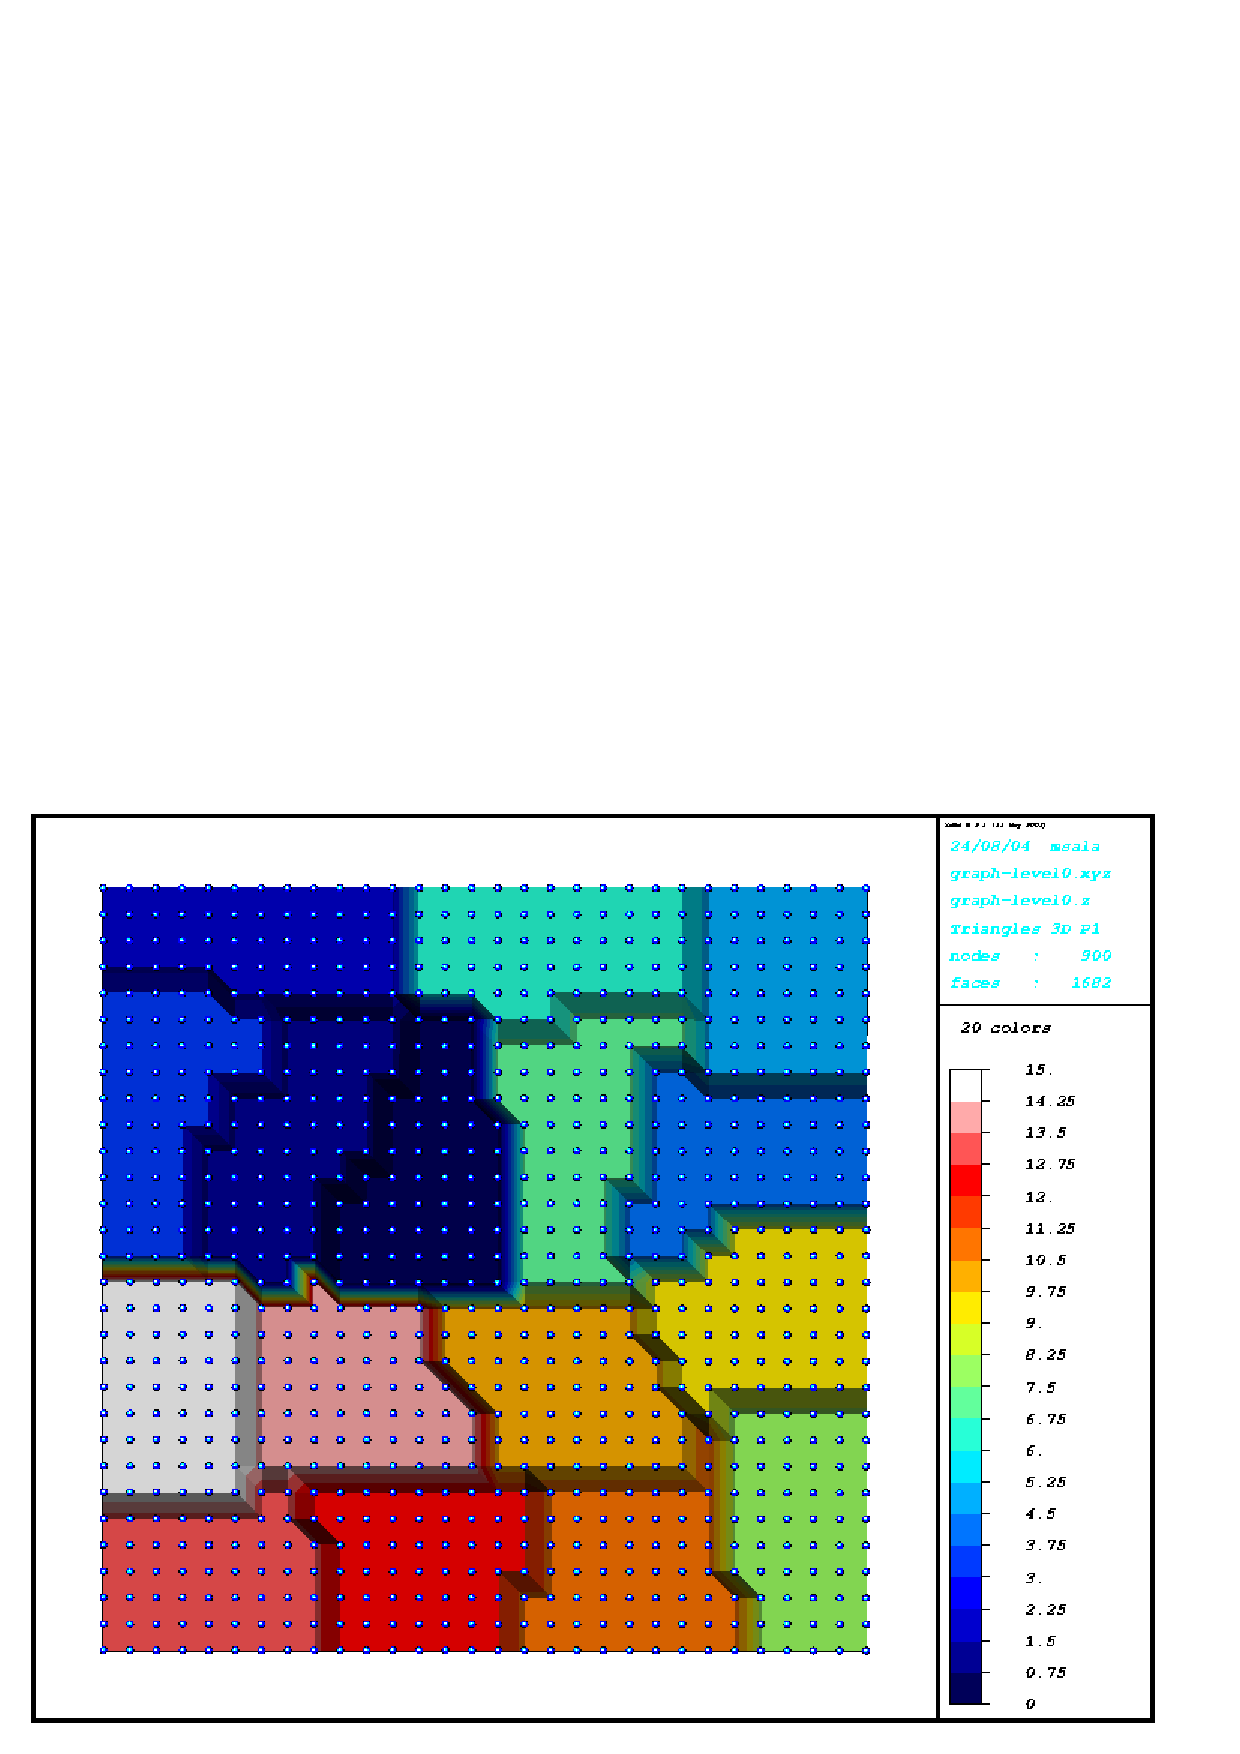
\includegraphics[width=12cm]{aggregate_decomposition}
\caption{Decomposition into aggregates. Uniform colors between blue spheres
represent the interior of aggregates.  Visualization was done with XD3D.}
\label{fig:viz:aggr}
\end{figure}

%%%
%%%
%%%

\subsubsection{Visualizing the effect of the \ML~Preconditioner and Smoothers}

In some cases, it may be useful to visualize the effect of the \ML~preconditioner, or of each level's smoother, on
a random vector (whose components are contained in the interval $[0.5,1]$), 
to understand if there are zones or directions that are not
affected by the current multilevel preconditioner. This can be easily 
done with the following code fragment:
\begin{verbatim}
double* x_coord;
double* y_coord;
// here we define the nodal coordinates...

MLList.set("viz: enable", true);
//you can also specify "xyz" on the line below
MLList.set("viz: output format", "vtk");
MLList.set("viz: x-coordinates", x_coord);
MLList.set("viz: y-coordinates", y_coord);
// by default the starting solution is not printed
MLList.set("viz: print starting solution", true);

// create the preconditioner
ML_Epetra::MultiLevelPreconditioner * MLPrec = 
  new ML_Epetra::MultiLevelPreconditioner(*A, MLList, true);

// visualize the effect of the ML preconditioner on a 
// random vector. We ask for 10 multilevel cycles
MLPrec->VisualizeCycle(10);

// visualize the effect of each level's smoother on a
// random vector. We ask for 5 steps of presmoothers,
// and 1 step of postsmoother
MLPrec->VisualizeSmoothers(5,1);
\end{verbatim}
(File \verb!ml_viz.cpp! contains the compilable
 code.) We note that the parameters must be set {\sl before} calling
{\tt ComputePreconditioner()}. See also Section~\ref{sec:MLP:auxiliary} for
the requirements on the coordinates vectors.
Results will be written in the following files:
\begin{itemize}
\item \verb!before-presmoother-eqX-levelY.vtk! contains the random vector
before
the application of the presmoother, for equation \verb!X! at level 
\verb!Y!;
\item \verb!after-presmoother-eqX-levelY.vtk! contains the random vector after
the application of the presmoother, for equation \verb!X! at level
\verb!Y!;
\item \verb!before-postsmoother-eqX-levelY.vtk! contains the random vector
before
the application of the postsmoother, for equation \verb!X! at level
\verb!Y!;
\item \verb!after-postsmoother-eqX-levelY.vtk! contains the random vector after
the application of the postsmoother, for equation \verb!X! at level
\verb!Y!;
\item \verb!before-cycle-eqX-levelY.vtk! contains the random vector
before
the application of the \ML cycle, for equation \verb!X! at the finest level;
\item \verb!after-cycle-eqX-levelY.vtk! contains the random vector after
the application of the ML cycle, for equation \verb!X! at finest level.
\end{itemize}

\begin{figure}[ht]
\centering
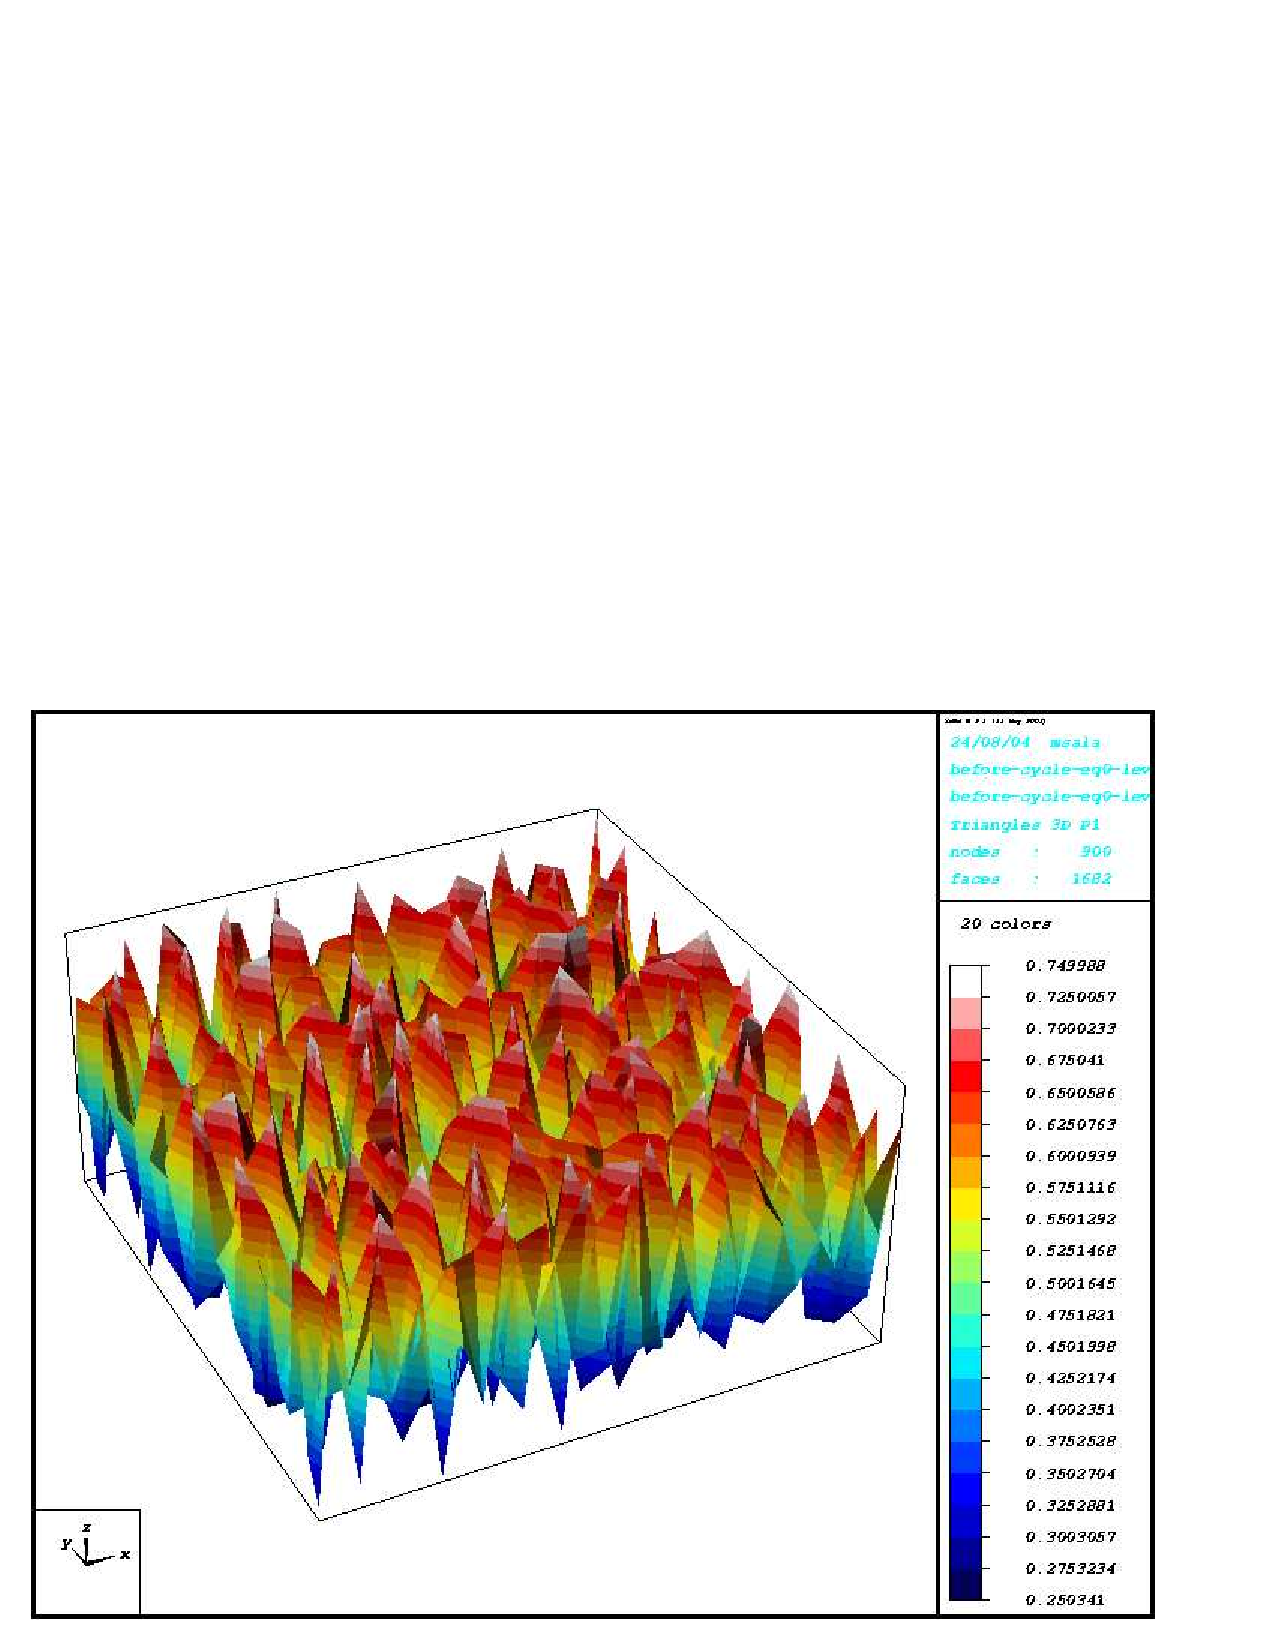
\includegraphics[width=7cm]{before_cycle} \hspace{0.5cm}
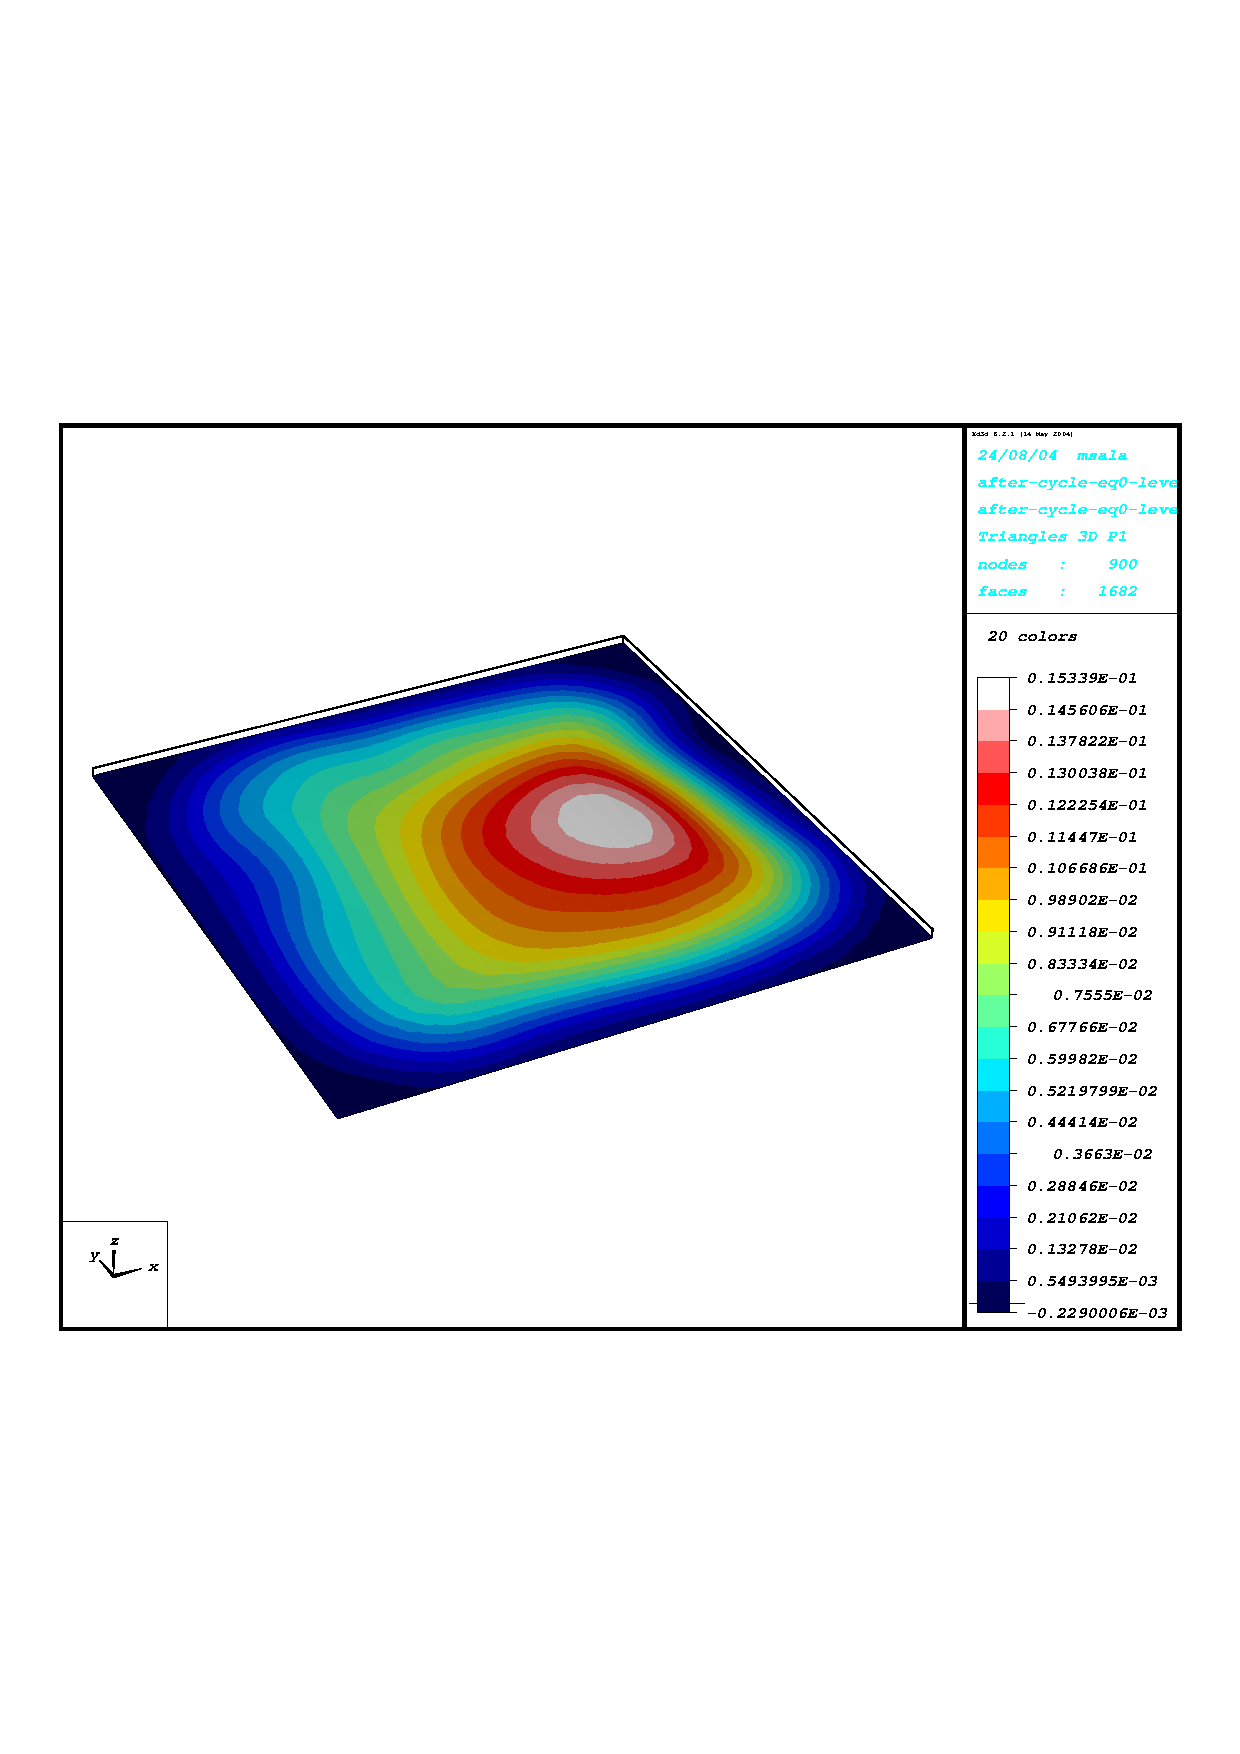
\includegraphics[width=7cm]{after_cycle}
\caption{Starting solution (left) and solution after 10 \ML~cycles (right).
Visualization was done using XD3D.}
\label{fig:viz:cycle}
\end{figure}

%%%
%%%
%%%

\subsection{Print the Computational Stencil for a 2D Cartesian Grid}

Method \verb!PrintStencil2D()! can be used to print out the computational
stencil for problems defined on 2D Cartesian grids, if the nodes numbering
follows the x-axis. The following fragment of code shows the use of this
method:
\begin{verbatim}
int Nx = 16; // nodes along the x-axis
int Ny = 32; // nodes along the y-axis
int NodeID = -1; // print the stencil for this node
int EquationID = 0; // equation 0, useful for vector problems

// MLPrec is a pointer to an already created 
// ML_Epetra::MultiLevelPreconditioner
MLPrec->PrintStencil2D(Nx,Ny,NodeID, EquationID);

// also valid in this case
MLPrec->PrintStencil2D(Nx,Ny);
\end{verbatim}
If \verb!NodeID == -1!, the code considers a node in the center of the
computational domain. The result can be something as follows:
\begin{verbatim}
2D computational stencil for equation 0 at node 136 (grid is 16 x 16)

                       0              -1               0
                      -1               4              -1
                       0              -1               0
\end{verbatim}

\clearpage
\newpage

%%%%%%%%%%%%%%%%%%%%%%%%%%%%%%%%%%%%%%%%%%%%%%%%%%%%%%%%%%
\section{Using the Maxwell Solvers in \ML} \label{maxwell solver}
%%%%%%%%%%%%%%%%%%%%%%%%%%%%%%%%%%%%%%%%%%%%%%%%%%%%%%%%%%
%
This section gives a brief overview of how to ML's two AMG preconditioners for
the eddy current formulation of Maxwell's equations.
These first solver (Maxwell) is intended only for real-valued
equations in the time domain.  The second solver (RefMaxwell) is intended for
real-valued (not complex) problems in the time or frequency domains.


\subsection{Background}\label{maxwell background}
The eddy current formulation of Maxwell's equations can be written as
\begin{equation} \label{maxwell pde}
\nabla\times\nabla\times \vec{E} + \sigma \vec{E} = \vec{f},
\end{equation}
where
$\vec{E}$\ is the unknown electric field to be computed,
$\sigma$ is the spatially-varying electrical conductivity,
and $\vec{f}$\ is the known right-hand side.
Neumann, Dirichlet, and/or periodic boundary conditions are supported.

Although we assume that (\ref{maxwell pde}) is discretized with
first-order edge elements, it is possible to use this preconditioner for
higher-order discretizations, as long as the user provides the sub-matrix
that corresponds to just the first-order discretization.
For more theoretical background and algorithm descriptions, please see
\cite{HTBGR_2004,BGHRT_2003}.

\subsection{Notational conventions}\label{maxwell notation}
For the remainder of the discussion, \Ke\ denotes the matrix corresponding to
the first-order element discretization of (\ref{maxwell pde}).   \Ke\ can be
written as
$$\Ke = S + M,$$
where $S$ is the stiffness matrix corresponding to the \curlcurl\ term in
(\ref{maxwell pde}), and $M$ is the mass matrix corresponding to the $\sigma\vec{E}$
term in (\ref{maxwell pde}).
The null-space of $S$ is given by the discrete gradient matrix, $T$.
$T$ corresponds to the null space of the \curlcurl\ term in
(\ref{maxwell pde}).
\Kn\ is an auxiliary nodal matrix that is described in \S\ref{Kn matrix}.


%%%%%%%%%%%%%%
\subsection{Description of the discrete gradient matrix $T$}\label{T matrix}
%%%%%%%%%%%%%%
%
$T$ is a rectangular, $N_e\times N_n$ matrix, where $N_e$ is the number of
edges in the mesh (rows in \Ke) and $N_n$ is the number of nodes in the mesh
(rows in \Kn).
Each row of $T$ has at most two entries, a $+1$ and/or a $-1$.
There are two ways to construct $T$.
In the first method, 
it's assumed that the mesh topology is available.
$T$ can be viewed as a node-edge incidence matrix of the mesh as a
directed graph.
As such,
each row of $T$ corresponds to an edge, and the $+1$/$-1$ entries in the
row are the head/tail of the edge, respectively.
Hence, $T$ can be built one row at a time by visiting each edge and inserting
$+1$/$-1$ in the appropriate columns.
The second method assumes that \Kn\ is already constructed.
Each off-diagonal nonzero entry, $(i,j)$, in the upper triangular
portion of \Kn\ corresponds to a row in $T$ containing
a $1$ and a $-1$ in columns $i$ and $j$.
%FIXME
%boundary conditions



%%%%%%%%%%%%%%
\subsection{Solver \#1: Maxwell}\label{maxwell:maxwell}
%%%%%%%%%%%%%%

The Maxwell solver is accessed through the
ML\_Epetra::MultiLevelPreconditioner class, which is described in more
detail in Section \ref{sec:getting_started}.

\subsubsection{Operators that the user must supply}
The user must provide three matrices:
\be
\item the first-order edge element matrix \Ke.
\item the auxiliary nodal matrix \Kn.
\item the discrete gradient matrix $T$.
\ee


%%%%%%%%%%%%%%
\subsubsection{Description of the auxiliary nodal matrix \Kn}\label{Kn matrix}
%%%%%%%%%%%%%%
%
\Kn\ is a square, $N_n\times N_n$ matrix, where $N_n$ is the number of nodes in
the mesh.
There are two ways to construct \Kn.
The first method is to discretize the PDE
\begin{equation}
   \int_\Omega \sigma u \cdot v + \int_\Omega \nabla u \cdot \nabla v,
   \label{nodal pde}
\end{equation}
using nodal linear finite elements on the same mesh as (\ref{maxwell pde}).
The second method assumes that you already have $T$ available.
\Kn\ can be formed via the triple-matrix product $$T^{\mathrm{T}}\Ke T =
T^{\mathrm{T}}M T,$$
where we have used the fact that $ST=0$.
%FIXME
%boundary conditions
%FIXME
%note consistency in parallel of how nodes, edges are distributed
%

%%%%%%%%%%%%%%
\subsubsection{Smoother options}\label{maxwell smoothers}
%%%%%%%%%%%%%%
%
The default smoother for the Maxwell solver is a two-stage smoother that we
call Hiptmair smoothing \cite{Hiptmair_1998a}.
This smoother consists of three steps: one step of a smoother $\mathcal S$ on
the entire system $Kx=f$; one step of a smoother $\mathcal S$ on the
projected system $T^{\mathrm{T}}MTe=T^{\mathrm{T}}r$, where $r = f - Kx$;
and finally one step of a smoother $\mathcal S$ on the entire system with
initial guess $x+e$.

The default sub-smoother $\mathcal S$ is a degree 3 Chebyshev
polynomial.
The coefficients of this polynomial are calculated automatically based on the
coarsening rate of the multigrid hierarchy.
The Chebyshev degree for the nodal (or edge) problem can be changed with the 
options \verb!subsmoother: node sweeps!  (or \verb!subsmoother: edge sweeps!)
and \verb!coarse: node sweeps! (or \verb!coarse: edge sweeps!) depending on
whether the Hiptmair smoothing is done on a fine or the coarsest level.

%%%%%%%%%%%%%%
\subsubsection{Sample Usage}\label{maxwell:maxwell example}
%%%%%%%%%%%%%%
\begin{verbatim}
#include "ml_MultiLevelPreconditioner.h"

// Allocate Matrices
Epetra_CrsMatrix CurlCurlMatrix(...);
Epetra_CrsMatrix TMatrix(...);
Epetra_CrsMatrix KnMatrix(...);

// Fill Matrices Here

// Build Maxwell Preconditioner
ML_Epetra::MultiLevelPreconditioner(CurlCurlMatrix, TMatrix, KnMatrix);
\end{verbatim}


%%%%%%%%%%%%%%
\subsection{Solver \#2: RefMaxwell}\label{maxwell:refmaxwell}
%%%%%%%%%%%%%%

The RefMaxwell solver is accessed through the
{\tt ML\_Epetra::RefMaxwellPreconditioner} class, which can be found in the
directory {\tt ml/src/RefMaxwell}.  This preconditioner handles the
range and null space of the curl operator with a dedicated
{\tt MultiLevelPreconditioner} object for each and has demonstrated
excellent parallel scalability in practice. The solver algorithm is
detailed in \cite{BHST_2007}

\subsubsection{Operators that the user must supply}
The user must provide four matrices:
\be
\item the first-order edge element matrix \Ke.
\item the discrete gradient matrix $T$.
\item the inverse of the (lumped) nodal mass matrix $\mathcal{M}_0$.
\item the edge mass matrix $\mathcal{M}_1$.
\ee

The matrices \Ke and $T$ are identical to the matrices used in Maxwell
(described in Section \ref{maxwell:maxwell}).  The matrix
$\mathcal{M}_0$ is used for the algebraic gauging of the edge space
and should include appropriate factors for the permeability ($\mu$).
The matrix $\mathcal{M}_1$ is used only for the edge space, meaning
that it does not include the conductivity ($\sigma$).

\subsubsection{Coarse nullspaces}
RefMaxwell will automatically calculate the nullspace for the coarse edge
problem from the discrete gradient matrix $T$ and nodal coordinates.
For periodic problems, however, this calculation will not be correct
(since the nodes on the periodic boundary are really in two places at
the same time).  In this case, the user can specify nullspace options
(using the standard syntax) as part of {\tt refmaxwell: 11list}.

\subsubsection{Smoother options}
Unlike the Maxwell solver, it is not particularly advantageous to use
the so-called Hiptmair hybrid smoother with RefMaxwell.  A more
traditional smoother, such as Chebyshev (in parallel) or Gauss-Seidel
(in serial) should be used.

\subsubsection{Setting parameter options}
RefMaxwell uses a nested parameter list in order to logically separate
the options for each individual solver.  Each sublist would include
the appropriate options for that particular solver.  A full list of
options supported by the {\tt MultiLevelPreconditioner} can be found
in Section~\ref{all possible parameters}.

In addition to the options for {\tt MultiLevelPreconditioner} (almost all
of which are valid), the RefMaxwell solver has the following unique options:

\choicebox{\tt refmaxwell: 11solver}{[{\tt string}] Sets the type of
  solver to use on the (1,1) block (edges).  Default: {\tt edge matrix free}.}

\choicebox{\tt refmaxwell: 11list}{[{\tt ParameterList}] Contains all
  of the options for the (1,1) block preconditioner (edges).}

\choicebox{\tt refmaxwell: 22solver}{[{\tt string}] Sets the type of
  solver to use on the (2,2) block (nodes).  Default: {\tt multilevel}.}

\choicebox{\tt refmaxwell: 22list}{[{\tt ParameterList}] Contains all
  of the options for the (2,2) block preconditioner (nodes).}

\choicebox{\tt refmaxwell: mode}{[{\tt string}] Sets the specific type
  of preconditioner used.  Default: {\tt additive}.}

\noindent The {\tt EdgeMatrixFreePreconditoner} for the (1,1)
block (currently the only supported option) also has one unique
option:

\choicebox{\tt edge matrix free: coarse}{[{\tt ParameterList}] Contains all
  of the options for the coarse (1,1) block preconditioner (edges).}


%%%%%%%%%%%%%
\subsubsection{Sample Usage}\label{maxwell:refmaxwell example}
%%%%%%%%%%%%%%
\begin{verbatim}
#include "ml_RefMaxwell.h"

// Allocate Matrices
Epetra_CrsMatrix CurlCurlMatrix(...);
Epetra_CrsMatrix TMatrix(...);
Epetra_CrsMatrix M0invMatrix(...);
Epetra_CrsMatrix M1Matrix(...);

// Fill Matrices Here

// Build RefMaxwell Preconditioner
ML_Epetra::RefMaxwellPreconditioner(CurlCurlMatrix, TMatrix,
                                    M0invMatrix, M1Matrix);
\end{verbatim}

\clearpage
\newpage

%%%%%%%%%%%%%%%%%%%%%%%%%%%%%%%%%%%%%%%%%%%%%%%%%%%%%%%%%%
\section{Advanced Usage of \ML} \label{high level sample}
%%%%%%%%%%%%%%%%%%%%%%%%%%%%%%%%%%%%%%%%%%%%%%%%%%%%%%%%%%
%
Sections~\ref{sec:getting_started} and ~\ref{all possible parameters} have detailed the
use of \ML~as a black box preconditioner. In some cases, instead, the
user may need to explicitly construct the \ML\ hierarchy. This is
reported in the following sections.

\medskip

A brief sample program is given in Figure \ref{high level figure}.
%
\begin{figure}[ht]
\begin{verbatim}

   ML_Create         (&ml_object, N_grids);

   ML_Init_Amatrix      (ml_object, 0,  nlocal, nlocal,(void *) A_data);
   ML_Set_Amatrix_Getrow(ml_object, 0,  user_getrow, NULL, nlocal_allcolumns);
   ML_Set_Amatrix_Matvec(ml_object, 0,  user_matvec);

   N_levels = ML_Gen_MGHierarchy_UsingAggregation(ml_object, 0, 
                                                  ML_INCREASING, NULL);
   ML_Gen_Smoother_Jacobi(ml_object, ML_ALL_LEVELS, ML_PRESMOOTHER, 1, 
                          ML_DEFAULT);
   ML_Gen_Solver    (ml_object, ML_MGV, 0, N_levels-1);
   ML_Iterate(ml_object, sol, rhs);
   ML_Destroy(&ml_object);
\end{verbatim}
\caption{High level multigrid sample code. \label{high level figure}}
\end{figure}
%
The function {\sf ML\_Create} creates a multilevel solver object that is
used to define the preconditioner. It requires the
maximum number of multigrid levels be specified. In
almost all cases, {\tt N\_grids}$ = 20$ is more than
adequate. The three `Amatrix' statements are used to define the 
discretization matrix, $A$, that is solved. This is discussed
in greater detail in Section \ref{single}. The 
multigrid hierarchy is generated via
{\sf ML\_Gen\_MGHierarchy\_UsingAggregation}. Controlling the behavior of
this function is discussed in Section \ref{aggregation options}.
For now, it is important
to understand that this function takes the matrix $A$ and sets up
relevant multigrid operators corresponding to the smoothed aggregation
multigrid method \cite{vanek3} \cite{vanek4}. In particular, it generates
a graph associated with $A$, coarsens this graph, builds functions
to transfer vector data between the original graph and
the coarsened graph, and then builds an approximation to $A$ on the
coarser graph. Once this second multigrid level is completed, the same
operations are repeated to the second level 
approximation to $A$ generating a third level. This process continues 
until the 
current graph is sufficiently coarse.  The function {\sf ML\_Gen\_Smoother\_Jacobi}
indicates that a Jacobi smoother should be used on all levels.
Smoothers are discussed further in Section \ref{multigrid options}.
Finally, {\sf ML\_Gen\_Solver} is invoked when the multigrid preconditioner
is fully specified. This function performs any needed initialization and
checks for inconsistent options. After {\sf ML\_Gen\_Solver} completes 
{\sf ML\_Iterate} can be used to solve the 
problem with an initial guess of {\tt sol} (which will be overwritten with
the solution) and a right hand side of {\tt rhs}. At the present time, the
external interface to vectors are just arrays. That is, {\tt rhs} and {\tt sol}
are simple one-dimensional arrays of the same length as the number of rows
in $A$. In addition to {\sf ML\_Iterate}, the function {\sf ML\_Solve\_MGV }
can be used to perform one multigrid `V' cycle as a preconditioner.

%%%
%%%
%%%

\section{Multigrid \& Smoothing Options} \label{multigrid options}
Several options can be set to tune the multigrid behavior.  In this
section, smoothing and high level multigrid choices are discussed. In
the next section, the more specialized topic of the grid transfer
operator is considered. 
%!@#The details of the functions described in these
%!@#next two sections are given in Section~\ref{subroutines}.

For most applications, smoothing choices are important to the overall performance
of the multigrid method.
Unfortunately, there is no simple advice as to what smoother will be
best and systematic experimentation is often necessary. \ML\ offers a variety 
of standard smoothers. Additionally, user-defined smoothers can be supplied
and it is possible to use \Aztec as a smoother.
A list of \ML\ functions that
can be invoked to use built-in smoothers are given below along with a 
few general comments.
\vskip .1in
\choicebox{ML\_Gen\_Smoother\_Jacobi} {
    Typically, not the fastest smoother.
    Should be used with damping. 
    For Poisson problems, the recommended damping values are 
    $\frac{2}{3}$ (1D), $\frac{4}{5}$ (2D), and $\frac{5}{7}$ (3D). In general, smaller damping numbers are
    more conservative.
}
\choicebox{ML\_Gen\_Smoother\_GaussSeidel}{
    Probably the most popular smoother. Typically, faster than Jacobi and
    damping is often not necessary nor advantageous. 
}
\choicebox{ML\_Gen\_Smoother\_SymGaussSeidel}{
    Symmetric version of Gauss Seidel. When using multigrid preconditioned 
    conjugate gradient, the multigrid operator must be symmetrizable. This
    can be achieved by using a symmetric smoother with the same number of
    pre and post sweeps on each level.
}
\choicebox{ML\_Gen\_Smoother\_BlockGaussSeidel}{
    Block Gauss-Seidel with a fixed block size.  Often used for PDE systems 
    where the block size is the number of degrees of freedom (DOFs) per grid point.
}
\choicebox{ML\_Gen\_Smoother\_VBlockJacobi}{
    Variable block Jacobi smoother. This allows users to specify unknowns
    to be grouped into different blocks when doing block Jacobi. 
}
\choicebox{ML\_Gen\_Smoother\_VBlockSymGaussSeidel}{
    Symmetric variable block Gauss-Seidel smoothing. This allows users to 
    specify unknowns to be grouped into different blocks when doing 
    symmetric block Gauss-Seidel. 
}
It should be noted that the parallel Gauss-Seidel smoothers are not true
Gauss-Seidel. In particular, each processor does a Gauss-Seidel iteration
using off-processor information from the previous iteration.
    
\Aztec~user's \cite{Aztec} can invoke {\sf ML\_Gen\_SmootherAztec} to use either
\Aztec~solvers or \Aztec~preconditioners as smoothers on any 
grid level. Thus, for example, it is possible to use preconditioned
conjugate-gradient (where the preconditioner might be an incomplete
Cholesky factorization) as a smoother within the multigrid method.
Using Krylov smoothers as a preconditioner could potentially be more
robust than using the simpler schemes provided directly by \ML.
However, one must be careful when multigrid is a preconditioner
to an outer Krylov iteration. Embedding an inner Krylov method within
a preconditioner to an outer Krylov method may not converge
due to the fact that the preconditioner can no longer be represented
by a simple matrix.
Finally, it is possible to pass user-defined smoothing functions into
\ML\ via {\sf ML\_Set\_Smoother}. The signature of the user defined
smoother function is
\begin{verbatim}

int user_smoothing(ML_Smoother *smoother, int x_length, double x[],
                   int rhs_length, double rhs[])

\end{verbatim}
where {\tt smoother} is an internal \ML\ object,
{\tt x} is a vector (of length {\tt x\_length}) that corresponds to the initial
guess on input and is the improved solution estimate on output, and {\tt rhs}
is the right hand side vector of length {\tt rhs\_length}. 
The function {\sf ML\_Get\_MySmootherData(smoother)} can be used to get
a pointer back to the user's data (i.e. the data pointer given with 
the {\sf ML\_Set\_Smoother} invocation). 
A simple (and suboptimal)
damped Jacobi smoother for the finest grid of our example is given below:
{\small 
\begin{verbatim}
int user_smoothing(ML_Smoother *smoother, int x_length, double x[], int rhs_length, double rhs[])
{
   int i;
   double ap[5], omega = .5; /* temp vector and damping factor */

   Poisson_matvec(ML_Get_MySmootherData(smoother), x_length, x, rhs_length, ap);
   for (i = 0; i < x_length; i++) x[i] = x[i] + omega*(rhs[i] - ap[i])/2.;

   return 0;
}
\end{verbatim} 
}
\noindent
A more complete smoothing example that operates on all multigrid levels
is given in the file \verb'mlguide.c'. This routine uses the functions
{\sf ML\_Operator\_Apply}, {\sf ML\_Operator\_Get\_Diag}, and {\sf
  ML\_Get\_Amatrix} to access coarse grid matrices constructed during
the algebraic multigrid process.  By writing these user-defined
smoothers, it is possible to tailor smoothers to a particular
application or to use methods provided by other packages.  In fact, the
\Aztec~methods within \ML\ have been implemented by writing wrappers to
existing \Aztec~functions and passing them into \ML\ via {\sf
  ML\_Set\_Smoother}.

At the present time there are only a few supported general parameters
that may be altered by users. However, we expect that this list will
grow in the future.  When using {\sf ML\_Iterate}, the convergence
tolerance ({\sf ML\_Set\_Tolerance}) and the frequency with which
residual information is output ({\sf ML\_Set\_ResidualOutputFrequency})
can both be set. Additionally, the level of diagnostic output from
either {\sf ML\_Iterate} or {\sf ML\_Solve\_MGV } can be set via {\sf
  ML\_Set\_OutputLevel}.  The maximum number of multigrid levels can be
set via {\sf ML\_Create} or {\sf ML\_Set\_MaxLevels}. Otherwise, \ML\
continues coarsening until the coarsest grid is less than or equal to a
specified size (by default 10 degrees of freedom).  This size can be set
via {\sf ML\_Aggregate\_Set\_MaxCoarseSize}.

\section{Smoothed Aggregation Options} \label{aggregation options}
When performing smooth aggregation, the matrix graph is first coarsened 
(actually vertices are aggregated together) and then a grid transfer
operator is constructed.  A number of parameters can be altered to
change the behavior of these phases. 

\subsection{Aggregation Options}

A graph of the matrix is usually constructed by associating a vertex
with each equation and adding an edge between two vertices $i$ and $j$
if there is a nonzero in the $(i,j)^{th}$ or $(j,i)^{th}$ entry. It is
this matrix graph whose vertices are aggregated together that effectively
determines the next coarser mesh. The above graph generation procedure
can be altered in two ways. First, a block matrix graph can be constructed
instead of a point matrix graph. In particular, all the degrees of freedom (DOFs) 
at a grid point
can be collapsed into a single vertex of the matrix graph. This situation
arises when a PDE system is being solved where each grid point has the same 
number of DOFs. The resulting block matrix graph is significantly smaller 
than the point matrix graph and by aggregating the block matrix graph, 
all unknowns at a grid point are kept together.  This usually results in
better convergence rates (and the coarsening is actually less expensive to 
compute).  To indicate the number of DOFs per node,
the function {\sf ML\_Aggregate\_Set\_NullSpace} is used.
The second way in which the graph matrix can be altered is by 
ignoring small values. In particular,
it is often preferential to ignore weak coupling during coarsening.
The error between weakly coupled points is generally hard to smooth
and so it is best not to coarsen in this direction.
For example,
when applying a Gauss-Seidel smoother to a standard discretization of 
$$
u_{xx} + \epsilon u_{yy} = f  
$$
(with $ 0 \le \epsilon \le 10^{-6}$) ,
there is almost no coupling in the $y$ direction. Consequently, simple smoothers
like Gauss-Seidel do not effectively smooth the error in this direction. If we apply a standard
coarsening algorithm, convergence rates suffer due to this lack of $y$-direction
smoothing. There are two principal ways to fix this: use a more sophisticated smoother
or coarsen the graph only in the $x$ direction.
By ignoring the $y$-direction coupling in the matrix graph, the aggregation phase 
effectively coarsens in only the $x$-direction (the direction
for which the errors are smooth)
yielding significantly better multigrid convergence rates. In general,
a drop tolerance,
$tol_{d}$,
can be set such that an individual matrix entry, $ A(i,j)$ is dropped
in the {\it coarsening phase}
if 
$$
 | A(i,j) | \le tol_d * \sqrt{ | A(i,i) A(j,j) | } .
 $$
 This drop tolerance (whose default value is zero) is set by {\sf
   ML\_Aggregate\_Set\_Threshold}.

There are two different groups of graph coarsening algorithms in \ML:
\begin{itemize}
\item schemes with fixed ratio of coarsening between levels: uncoupled
  aggregation, coupled aggregation, and MIS aggregation.  A description
  of those three schemes along with some numerical results are given in
  \cite{supercomputing}. As the default, the {\tt Uncoupled-MIS} scheme is used which
  does uncoupled aggregation on finer grids and switches to the more
  expensive MIS aggregation on coarser grids;
\item schemes with variable ratio of coarsening between levels:
  \metis~and \parmetis aggregation. Those schemes use the graph
  decomposition algorithms provided by \metis~and \parmetis, to create
  the aggregates.
\end{itemize}
Poorly done aggregation can adversely affect the multigrid convergence
and the time per iteration. In particular, if the scheme coarsens too
rapidly multigrid convergence may suffer. However, if coarsening is too
slow, the number of multigrid levels increases and the number of
nonzeros per row in the coarse grid discretization matrix may grow
rapidly. We refer the reader to the above paper and indicate that users
might try experimenting with the different schemes via {\sf
  ML\_Aggregate\_Set\_CoarsenScheme\_Uncoupled}, {\sf
  ML\_Aggregate\_Set\_CoarsenScheme\_Coupled}, \newline {\sf
  ML\_Aggregate\_Set\_CoarsenScheme\_MIS}, {\sf
  ML\_Aggregate\_Set\_CoarsenScheme\_METIS}, and \\ {\sf
  ML\_Aggregate\_Set\_CoarsenScheme\_ParMETIS}.

%Finally, within the uncoupled and border aggregation it is possible to 
%set the following ...

\subsection{Interpolation Options}
An interpolation operator is built using coarsening information,
seed vectors, and a damping factor. We refer the 
reader to \cite{vanek4} for details on the algorithm and the theory. 
In this section, we explain a few essential features to
help users direct the interpolation process. 

Coarsening or aggregation information is first used to create a
tentative interpolation operator.  This process takes a seed vector or
seed vectors and builds a grid transfer operator. The details of this
process are not discussed in this document.  It is, however, important
to understand that only a few seed vectors are needed (often but not
always equal to the number of DOFs at each grid point) and that these
seed vectors should correspond to components that are difficult to
smooth.  The tentative interpolation that results from these seed
vectors will interpolate the seed vectors perfectly.  It does this by
ensuring that all seed vectors are in the range of the interpolation
operator.  This means that each seed vector can be recovered by
interpolating the appropriate coarse grid vector.  The general idea of
smoothed aggregation (actually all multigrid methods) is that errors not
eliminated by the smoother must be removed by the coarse grid solution
process.  If the error after several smoothing iterations was known, it
would be possible to pick this error vector as the seed vector. However,
since this is not the case, we look at vectors associated with small
eigenvalues (or singular values in the nonsymmetric case) of the
discretization operator.  Errors in the direction of these eigenvectors
are typically difficult to smooth as they appear much smaller in the
residual ($ r = A e $ where $r$ is the residual, $A$ is discretization
matrix, and $e$ is the error).  For most scalar PDEs, a single seed
vector is sufficient and so we seek some approximation to the
eigenvector associated with the lowest eigenvalue.  It is well known
that a scalar Poisson operator with Neumann boundary conditions is
singular and that the null space is the constant vector. Thus, when
applying smoothed aggregation to Poisson operators, it is quite natural
to choose the constant vector as the seed vector.  In many cases, this
constant vector is a good choice as all spatial derivatives within the
operator are zero and so it is often associated with small singular
values. Within \ML\ the default is to choose the number of seed vectors
to be equal to the number of DOFs at each node (given via {\sf
  ML\_Aggregate\_Set\_NullSpace}).  Each seed vector corresponds to a
constant vector for that DOF component.  Specifically, if we have a PDE
system with two DOFs per node. Then one seed vector is one at the first
DOF and zero at the other DOF throughout the graph. The second seed
vector is zero at the first DOF and one at the other DOF throughout the
graph.  In some cases, however, information is known as to what
components will be difficult for the smoother or what null space is
associated with an operator.  In elasticity, for example, it is well
known that a floating structure has six rigid body modes (three
translational vectors and three rotation vectors) that correspond to the
null space of the operator.  In this case, the logical choice is to take
these six vectors (which can be computed with the help of {\tt ML\_Coord2RBM()}) 
as the seed vectors in smoothed aggregation. When this
type of information is known, it should be given to \ML\ via the command
{\sf ML\_Aggregate\_Set\_NullSpace}.

Once the tentative prolongator is created, it is smoothed via a damped Jacobi
iteration. The reasons for this smoothing are related to the theory where the
interpolation basis functions must have a certain degree of smoothness (see \cite{vanek4}).
However, the smoothing stage can be omitted by setting the damping to zero
using the function 
{\sf ML\_Aggregate\_Set\_DampingFactor}. Though
theoretically poorer, unsmoothed aggregation can have considerably less set up
time and less cost per iteration than smoothed aggregation.
When smoothing,
\ML\ has a few ways to determine the Jacobi damping parameter and each 
require some estimate of the spectral radius of the discretization 
operator. The current default is to use a few iterations of the power method
method (subspace size of two) to estimate this value
(see {\sf ML\_Set\_SpectralNormScheme\_PowerMethod}) However, if the
matrix is symmetric conjugate-gradient method should be used via
{\sf ML\_Set\_SpectralNormScheme\_Calc}. It is also possible to
change the default number of iterations used in the eigensolver from
ten via {\sf ML\_Set\_SpectralNorm\_Iterations}. 
There are several other internal parameters that have not 
been discussed in this document. In the future, it is anticipated that some of 
these will be made available to users.


%
%%%%%%%%%%%%%%%%%%%%%%%%%%%%%%%%%%%%%%%%%%%%%%%%%%%%%%%%%%
\section{Advanced Usage of \ML\ and Epetra}
\label{sec:advanced}
%%%%%%%%%%%%%%%%%%%%%%%%%%%%%%%%%%%%%%%%%%%%%%%%%%%%%%%%%%
%
Class ML\_Epetra::MultiLevelOperator is defined in a header file, that must
be included as
\begin{verbatim}
#include "ml_MultiLevelOperator.h" 
\end{verbatim}
Users may also need to include \verb!ml_config.h!,
\verb!Epetra_Operator.h!, \verb!Epetra_MultiVector.h!,
\verb!Epetra_LinearProblem.h!,  \verb!AztecOO.h!. Check the {\sc Epetra} and
AztecOO documentation for more details.

Let \verb!A! be an Epetra\_RowMatrix for which we aim to construct
a preconditioner, and let \verb!ml_handle! be the structure \ML\ requires
to store internal data (see Section~\ref{high level sample}), created
with the instruction
\begin{verbatim}
ML_Create(&ml_handle,N_levels);
\end{verbatim}
where \verb!N_levels! is the specified (maximum) number of levels.  As
already pointed out, \ML\ can accept in input very general matrices.
Basically, the user has to specify the number of local rows, and provide
a function to update the ghost nodes (that is, nodes requires in the
matrix-vector product, but assigned to another process). For Epetra
matrices, this is done by the following function
\begin{verbatim}
EpetraMatrix2MLMatrix(ml_handle, 0, &A);
\end{verbatim}
and it is important to note that \verb!A! is {\sl not} converted to ML
format. Instead, {\sf EpetraMatrix2MLMatrix} defines a suitable getrow
function (and other minor data structures) that allows \ML\ to work with
\verb!A!.

Let \verb!agg_object! a ML\_Aggregate pointer, created using
\begin{verbatim}
ML_Aggregate_Create(&agg_object);
\end{verbatim}
At this point, users have to create the multilevel hierarchy, define the
aggregation schemes, the smoothers, the coarse solver, and create the solver.
Then, we can finally create the ML\_Epetra::MultiLevelOperator object
\begin{verbatim}
ML_Epetra::MultiLevelOperator MLop(ml_handle,comm,map,map);
\end{verbatim}
(\verb!map! being the Epetra\_Map used to create the matrix) and set the
preconditioning operator of our {\sc AztecOO} solver,
\begin{verbatim}
Epetra_LinearProblem Problem(A,&x,&b);
AztecOO Solver(Problem);
solver.SetPrecOperator(&MLop);
\end{verbatim}
where \verb!x! and \verb!b! are \verb!Epetra_MultiVector!'s defining
solution and right-hand side. The linear problem can now be solved as,
for instance,
\begin{verbatim}
Solver.SetAztecOption( AZ_solver, AZ_gmres );
solver.Iterate(Niters, 1e-12);
\end{verbatim}

%%%
%%%
%%%

\section{Using \ML\ without Epetra}
\label{sec:without_Epetra}

\subsection{Creating a \ML\ matrix: Single Processor}
\label{single}

Matrices are created by defining some size information, a matrix-vector
product and a getrow function (which is used to extract matrix
information).  We note that {\sc Epetra} and {\sc Aztec} users do not
need to read this (or the next) section as there are special functions
to convert {\sc Epetra} objects and {\sc Aztec} matrices to \ML\ matrices (see
Section \ref{other packages}). Further, functions for
some common matrix storage formats (CSR \& MSR) already exist within ML
and do not need to be rewritten\footnote{The functions {\sf
    CSR\_matvec}, {\sf CSR\_getrows}, {\sf MSR\_matvec} and {\sf
    MSR\_getrows} can be used.}.

Size information is indicated via {\sf ML\_Init\_Amatrix}. The third parameter
in the Figure \ref{high level figure} 
invocation
indicates that a matrix with {\tt nlocal} rows is being defined. The fourth parameter
gives the vector length of vectors that can be multiplied with this matrix.  
Additionally,
a data pointer, {\tt A\_data}, is associated with the matrix. This pointer 
is passed back into the matrix-vector product and getrow functions that are 
supplied by the user. Finally, the number `0' indicates at what level within
the multigrid hierarchy the matrix is to be stored. For discussions within this
document, this is always `0'. It should be noted that there appears to be some redundant
information. In particular, the number of rows and the vector length in
{\sf ML\_Init\_Amatrix} should be the same number as the discretization matrices are square.
Cases where these `apparently' redundant parameters might be set differently
are not discussed in this document.

The function {\sf ML\_Set\_Amatrix\_Matvec} associates a 
matrix-vector product with the discretization matrix.
The invocation in Figure
\ref{high level figure} indicates that the matrix-vector product
function
{\tt user\_matvec} is associated with the matrix located at level
`{\tt 0}' of the multigrid hierarchy.  The signature of {\tt user\_matvec} is
%
\begin{verbatim}
int user_matvec(ML_Operator *Amat, int in_length, double p[], int out_length, 
                double ap[])
\end{verbatim}
%
where {\tt A\_mat} is an internal \ML\ object,
%the user-defined data pointer specified in the 
%{\sf ML\_Init\_Amatrix}, 
{\tt p} is the vector to apply to the matrix,
{\tt in\_length} is the length of this vector, and {\tt ap} is the 
result after
multiplying the discretization matrix by the vector {\tt p} 
and {\tt out\_length}
is the length of {\tt ap}.
The function {\sf ML\_Get\_MyMatvecData(Amat)} can be used to get
a pointer back to the user's data (i.e. the data pointer given with 
the {\sf ML\_Init\_Amatrix} invocation). 

Finally, {\sf ML\_Set\_Amatrix\_Getrow} associates a getrow function with 
the discretization matrix.  This getrow function returns nonzero information 
corresponding to specific rows.  
The invocation 
in Figure \ref{high level figure}
indicates that a user supplied function {\tt user\_getrow} is 
associated with the matrix located at level `{\tt 0}' of the multigrid
hierarchy and that this matrix contains {\tt nlocal\_allcolumns} columns 
and that no communication ({\tt NULL})
is used (discussed in the next section).
It again appears that some redundant information is being asked as the 
number of columns was already given. However, when running in parallel
this number will include ghost node information and is usually different
from the number of rows.
The signature of {\tt user\_getrow} is
%
\begin{verbatim}
int user_getrow(ML_Operator *Amat, int N_requested_rows, int requested_rows[],
   int allocated_space, int columns[], double values[], int row_lengths[])
\end{verbatim}
%
where {\tt Amat} is an internal \ML\ object,
{\tt N\_requested\_rows} is the number of matrix rows for which 
information is
returned, {\tt requested\_rows} are the specific rows for which information will be returned,
{\tt allocated\_space} indicates how much space has been allocated in 
{\tt columns}
and {\tt values} for nonzero information. 
The function {\sf ML\_Get\_MyGetrowData(Amat)} can be used to get
a pointer back to the user's data (i.e. the data pointer given with 
the {\sf ML\_Init\_Amatrix} invocation). On return, the user's function
should take each row in order within {\tt requested\_rows} and place the 
column numbers and the values corresponding to nonzeros in the 
arrays {\tt columns} and {\tt values}. The length of the ith requested row
should appear in {\tt row\_lengths[i]}. If there is not enough allocated 
space in {\tt columns} or {\tt values}, this routine simply returns a `{\tt 0}',
otherwise it returns a `{\tt 1}'.


To clarify, these functions, one concrete example is given
corresponding to the matrix:
\begin{equation} \label{matrix example}
\pmatrix{ 2 & -1 &    &    &    \cr
         -1 &  2 & -1 &    &    \cr
            & -1 &  2 & -1 &    \cr
            &    & -1 &  2 & -1 \cr
            &    &    & -1 &  2 } .
\end{equation}
To implement this matrix, the following functions are defined:
%
{\small
\begin{verbatim}
int Poisson_getrow(ML_Operator *Amat, int N_requested_rows, int requested_rows[],
   int allocated_space, int columns[], double values[], int row_lengths[])
{
   int count = 0, i, start, row;


   for (i = 0; i < N_requested_rows; i++) {
      if (allocated_space < count+3) return(0);
      start = count;
      row = requested_rows[i];
      if ( (row >= 0) || (row <= 4) ) {
         columns[count] = row; values[count++] = 2.;
         if (row != 0) { columns[count] = row-1; values[count++] = -1.; }
         if (row != 4) { columns[count] = row+1; values[count++] = -1.; }
      }
      row_lengths[i] = count - start;
   }
   return(1);
}
\end{verbatim}
}
%
\noindent
and
%
{\small
\begin{verbatim}
int Poisson_matvec(ML_Operator *Amat, int in_length, double p[], int out_length, 
                   double ap[])
{
   int i;

   for (i = 0; i < 5; i++ ) {
      ap[i] = 2*p[i];
      if (i != 0) ap[i] -= p[i-1];
      if (i != 4) ap[i] -= p[i+1];
   }
   return 0;
}
\end{verbatim}
}
%
\noindent
Finally, these matrix functions along with size information are associated with the
fine grid discretization matrix via
\begin{verbatim}
   ML_Init_Amatrix      (ml_object, 0,  5, 5, NULL);
   ML_Set_Amatrix_Getrow(ml_object, 0,  Poisson_getrow, NULL, 5);
   ML_Set_Amatrix_Matvec(ml_object, 0,  Poisson_matvec);
\end{verbatim}
Notice that in these simple examples {\tt Amat} was not used.
In the next section we give a parallel example which makes use of 
{\tt Amat}. The complete sample program can be found in the
file \verb'mlguide.c' within the \ML\ code distribution.

\subsection{Creating a \ML\ matrix: Multiple Processors} 
\label{sec:multiple}

Creating matrices in parallel requires a bit more work. In this
section local versus global indexing as well as communication
are discussed.  In the description, we reconsider the previous example 
(\ref{matrix example}) partitioned over two processors. 
The matrix row indices (ranging from 0 to 4) are referred to as global 
indices and are independent of the number of processors being used.
On distributed memory machines, the matrix is subdivided
into pieces that are assigned to individual processors.  \ML\ 
requires matrices be partitioned by rows (i.e. each row is 
assigned to a processor which holds the entire data for that row).
These matrix pieces are stored on each processor as smaller local 
matrices. Thus, global indices in the original matrix get mapped to
local indices on each processor.
In our
example, we will assign global rows 0 and 4 to processor 0 
and store them locally as rows 1 and 0 respectively.
Global columns 0, 1, 3,  and 4 are stored locally as columns 1, 3, 2, and
0. This induces the local matrix
$$
\pmatrix{2 &  & -1  &  \cr     & 2 & & -1 } .
$$
Likewise, processor 1 is assigned global rows 1, 2, and 3 which are
stored locally as rows 0, 1, and 2 respectively.
Global columns 0 - 4 are stored locally as columns 3, 0, 1, 2, and 4
inducing the local matrix 
$$
\pmatrix{2 & -1 &    &     & -1 \cr
        -1 & 2  & -1 &     &    \cr 
           & -1 & 2  & -1  &     } .
$$
At the present time, there are some restrictions
as to what type of mappings can be used. In particular, all global rows 
stored on a processor must be mapped from 0 to $k-1$ where $k$ is the
number of rows assigned to this processor. This row mapping induces a
partial column mapping. Any additional columns must be mapped with
consecutive increasing numbers starting from $k$.

\ML\ has no notion of global indices and uses only the local indices.
In most cases, another package or application already mapped
the global indices to local indices and so 
\ML\ works with the existing local
indices.  Specifically, the parallel version of 
{\tt user\_getrow} and {\tt user\_matvec} should correspond
to each processor's local matrix.  This means that when giving
the column information with {\sf ML\_Set\_Amatrix\_Getrow}, the
total number of columns in the local matrix should be given and that
when row $k$ is requested, {\tt user\_getrow} should return the $k^{th}$ local
row using local column indices. Likewise, the matrix-vector product
takes a local input vector and multiplies it by the local
matrix. It is important to note that this local input vector
does not contain ghost node data
(i.e. the input vector is of length {\tt nlocal} where {\tt nlocal} is the number of matrix rows). 
Thus, 
{\tt user\_matvec} must perform the necessary communication to update
ghost variables.  When invoking {\sf ML\_Init\_Amatrix}, the local number of rows 
should be given for the number of rows and the vector 
length\footnote{ In contrast to {\sf ML\_Set\_Amatrix\_Getrow} in which the number of
local columns are given (including those that correspond to ghost variables), 
{\sf ML\_Init\_Amatrix} does not include ghost variables and so both size parameters
should be the number of local rows.}.
A specific communication
function must also be passed into \ML\ when supplying the getrow function
so that \ML\ can determine how local 
matrices on different processors are `glued' together.
The signature of the communication function is
%
\begin{verbatim}
int user_comm(double x[], void *Adata) 
\end{verbatim}
%
where {\tt A\_data} is the user-defined data pointer specified in the
{\sf ML\_Init\_Amatrix} and {\tt x} is a vector of length 
{\tt nlocal\_allcolumns} specified in {\sf ML\_Set\_Amatrix\_Getrow}. This parameter
should be set to the total number of matrix columns stored on this processor.
On input, only the first {\tt nlocal} elements of {\tt x} are
filled with data where {\tt nlocal} is the number of rows/columns specified
in {\sf ML\_Init\_Amatrix}. On output, the ghost elements 
are updated to their current values (defined on other processors). Thus, after 
this function a local matrix-vector product could be properly performed
using {\tt x}. To make all this clear, we give the new functions 
corresponding to our two processor example.

{\small
\begin{verbatim}
int Poisson_getrow(ML_Operator *Amat, int N_requested_rows, int requested_rows[],
   int allocated_space, int cols[], double values[], int row_lengths[])
{
   int m = 0, i, row, proc, *itemp, start;

   itemp = (int *) ML_Get_MyGetrowData(Amat);
   proc  = *itemp;

   for (i = 0; i < N_requested_rows; i++) {
      row = requested_rows[i];
      if (allocated_space < m+3) return(0);
      values[m] = 2; values[m+1] = -1; values[m+2] = -1;
      start = m;
      if (proc == 0) {
         if (row == 0) {cols[m++] = 0; cols[m++] = 2;               }
         if (row == 1) {cols[m++] = 1; cols[m++] = 3;}
      }
      if (proc == 1) {
         if (row == 0) {cols[m++] = 0; cols[m++] = 1; cols[m++] = 4;}
         if (row == 1) {cols[m++] = 1; cols[m++] = 0; cols[m++] = 2;}
         if (row == 2) {cols[m++] = 2; cols[m++] = 1; cols[m++] = 3;}
      }
      row_lengths[i] = m - start;
   }
   return(1);
}
\end{verbatim}
}
%
%
{\small
\begin{verbatim}
int Poisson_matvec(ML_Operator *Amat, int in_length, double p[], int out_length, 
                   double ap[])
{
   int i, proc, *itemp;
   double new_p[5];

   itemp = (int *) ML_Get_MyMatvecData(Amat);
   proc  = *itemp;

   for (i = 0; i < in_length; i++) new_p[i] = p[i];
   Poisson_comm(new_p, A_data);

   for (i = 0; i < out_length; i++) ap[i] = 2.*new_p[i];

   if (proc == 0) {
      ap[0] -= new_p[2];
      ap[1] -= new_p[3];
   }
   if (proc == 1) {
      ap[0] -= new_p[1]; ap[0] -= new_p[4];
      ap[1] -= new_p[2]; ap[1] -= new_p[0];
      ap[2] -= new_p[3]; ap[2] -= new_p[1];
   }
   return 0;
}
\end{verbatim}
}
and
{\small
\begin{verbatim}
int Poisson_comm(double x[], void *A_data)
{
   int    proc, neighbor, length, *itemp;
   double send_buffer[2], recv_buffer[2];

   
   itemp = (int *) A_data;
   proc  = *itemp; 

   length = 2;
   if (proc == 0) {
      neighbor = 1;
      send_buffer[0] = x[0]; send_buffer[1] = x[1];
      send_msg(send_buffer,  length, neighbor);
      recv_msg(recv_buffer,  length, neighbor);
      x[2] = recv_buffer[1]; x[3] = recv_buffer[0];
   }
   else {
      neighbor = 0;
      send_buffer[0] = x[0]; send_buffer[1] = x[2];
      send_msg(send_buffer,  length, neighbor);
      recv_msg(recv_buffer,  length, neighbor);
      x[3] = recv_buffer[1]; x[4] = recv_buffer[0];
   }
   return 0;
}
\end{verbatim}
}
\noindent
Finally, these matrix functions along with size information are associated with the
fine grid discretization matrix via
\begin{verbatim}
   if     (proc == 0) {nlocal = 2; nlocal_allcolumns = 4;}
   else if (proc == 1) {nlocal = 3; nlocal_allcolumns = 5;}
   else               {nlocal = 0; nlocal_allcolumns = 0;}

   ML_Init_Amatrix      (ml_object, 0,  nlocal, nlocal, &proc);
   ML_Set_Amatrix_Getrow(ml_object, 0,  Poisson_getrow, Poisson_comm, 
                         nlocal_allcolumns);
   ML_Set_Amatrix_Matvec(ml_object, 0,  Poisson_matvec);
\end{verbatim}



%%%%%%%%%%%%%%%%%%%%%%%%%%%%%%%%%%%%%%%%%%%%%%%%%%%%%%%%%%
\section{MLMEX: The MATLAB Interface for ML} \label{sec:mlmex}
%%%%%%%%%%%%%%%%%%%%%%%%%%%%%%%%%%%%%%%%%%%%%%%%%%%%%%%%%%
MLMEX is ML's interface to the MATLAB environment.  It allows access
to a limited set of routines either using the ML\_Epetra or the MLAPI
interfaces.  It is designed to provide access to ML's aggregation and
solver routines from MATLAB and does little else.  MLMEX allows users
to setup and solve arbitrarily many problems, so long as memory
suffices.  More than one problem can be setup simultaneously. 

\subsection{Autotools Configure and Make}\label{sec:mlmex:conf_make}
WARNING: Autotools support was deprecated with Trilinos 10.0.  There
is no guarantee that this will work with any Trilinos 10.0 or beyond.
See Section~\ref{sec:mlmex:cmake} for building MLMEX with cmake.

In order to use MLMEX, ML must be configured with (at least) the following options:
\begin{verbatim}
../configure -enable-epetra --enable-teuchos --enable-ifpack \
  --enable-aztecoo --enable-galeri --enable-amesos --enable-epetraext \
  --enable-ml-matlab \
  --with-matlab-exec=<directory with matlab binaries> \
  --with-matlab-root=<root directory of matlab install>
\end{verbatim}
Most additional options (such as \texttt{--enable-zoltan}) can be specified
as well.  It is important to note that MLMEX does not work properly
with MPI, hence MPI must be disabled in order to compile MLMEX .

On 64-bit Intel/AMD architectures, ML and all required Trilinos
libraries must be compiled with the \texttt{-fPIC} option.  This
necessitates adding \verb!CFLAGS=-fPIC CXXFLAGS=-fPIC FFLAGS=-fPIC! to
the Trilinos configure line.  Currently, MLMEX will not compile under
Solaris. 

The build system uses the \texttt{mexext} script from Mathworks to
detect the appropriate file extension for the architecture.  At
present, this means that cross-compilation is not possible.  It also
means that MLMEX will only support MATLAB 7.2 (R2006a) and up.


\subsection{Cmake Configure and Make}\label{sec:mlmex:cmake}
To use MLMEX, Trilinos must be configured with (at least) the
following options:

\begin{verbatim}
cmake \
-D Trilinos_ENABLE_Amesos:BOOL=ON \
-D Trilinos_ENABLE_AztecOO:BOOL=ON \
-D Trilinos_ENABLE_Epetra:BOOL=ON \
-D Trilinos_ENABLE_EpetraExt:BOOL=ON \
-D Trilinos_ENABLE_Ifpack:BOOL=ON \
-D Trilinos_ENABLE_ML:BOOL=ON \
-D Trilinos_ENABLE_Teuchos:BOOL=ON \
-D MATLAB_ROOT:STRING="<directory of matlab root>" \
-D MATLAB_ARCH:STRING="<matlab arch>" \
-D TPL_ENABLE_MATLAB:BOOL=ON \
../Trilinos
\end{verbatim}
Most additional options can be specified as well.  It is important to
note that MLMEX does not work properly with MPI, hence MPI must be
disabled in order to compile MLMEX.  The MATLAB\_ARCH option is new to
the cmake build system, and involves the MATLAB-specific architecture
code for your system.  There is currently no automatic way to extract
this, so it must be user-specified.  As of MATLAB 7.9 (R2009b), common
arch codes are:
\begin{center}
\begin{tabular}{l|l}
Code& OS\\
\hline
glnx86& 32-bit Linux (intel/amd)\\
glnxa64& 64-bit Linux (intel/amd)\\
sol64& 64-bit Solaris(sparc)\\
sola64& 64-bit Solaris(intel/amd)\\
maci64& 64-bit MacOS\\
maci& 32-bit MacOS\\
\end{tabular}
\end{center}

On 64-bit Intel/AMD architectures, Trilinos and all relevant TPLs
(note: this includes BLAS and LAPACK)
must be compiled with the \texttt{-fPIC} option.  This necessitates adding:
\begin{verbatim}
-D CMAKE_CXX_FLAGS:STRING="-fPIC" \
-D CMAKE_C_FLAGS:STRING="-fPIC" \
-D CMAKE_Fortran_FLAGS:STRING="-fPIC" \
\end{verbatim}
to the cmake configure line.  Trilinos does not play nicely with
MATLAB's default LAPACK and BLAS on 64-bit machines, so be sure to
specify your own with something like:
\begin{verbatim}
-D LAPACK_LIBRARY_DIRS:STRING="<path to my lapack>" \
-D BLAS_LIBRARY_DIRS:STRING="<path to my blas>" \
\end{verbatim}
If MLMEX randomly crashes when you turn 'PDE equations' above one,
chances are MLMEX is finding the wrong BLAS/LAPACK libraries.  Be sure
cmake is finding the right copy. MLMEX has only been tested with cmake on MATLAB 7.9 (R2009b) on a
64-bit Linux system.  Like the autotools build, the cmake uses
\texttt{mexext}, so any version of MATLAB before version 7.2 (R2006a)
will never work.  MLMEX is also unlikely to work on Solaris.


\subsection{Using MLMEX}\label{sec:mlmex:usage}
MLMEX is designed to be interfaced with via the MATLAB script
\texttt{ml.m}.  There are five modes in which MLMEX can be run:
\begin{enumerate}
\item Setup Mode --- Performs the problem setup for ML.
  Depending on whether or not the \texttt{mlmex: interface} option is
  used, MLMEX creates either a ML\_Epetra or MLAPI object.  This call
  returns a problem handle used to reference the problem in the future.
\item Solve Mode --- Given a problem handle and a right-hand side, ML
  solves the problem specified.  Setup mode must be called before
  solve mode.
\item Cleanup Mode --- Frees the memory allocated to internal ML
  objects.  This can be called with a particular problem handle, in
  which case it frees that problem, or without one, in which case all
  MLMEX memory is freed.
\item Status Mode --- Prints out status information on problems which
  have been set up.  Like cleanup, it can be called with or without a
  particular problem handle.
\item Aggregate Mode --- Uses MLMEX as an interface to ML's
  aggregation routines. 
\end{enumerate}
All of these modes, with the exception of status and cleanup take
option lists which will be directly converted into
\texttt{Teuchos::ParameterList} objects by MLMEX.  This means that 
the options described in Section~\ref{sec:getting_started} for
ML\_Epetra and those in the MLAPI guide (for MLAPI) will work
correctly for MLMEX. 

\subsubsection{Setup Mode}
Setup mode is called as follows:
\begin{verbatim}
>> [h,oc]=ml('setup',A,['parameter',value,...]) 
\end{verbatim}
The parameter \texttt{A} represents the sparse matrix to perform aggregation on
and the parameter/value pairs represent standard ML options.

The routine returns a problem handle, \texttt{h}, and the operator
complexity \texttt{oc} for the operator.  In addition to the standard
options, setup mode has one unique option of its own:

\choicebox{\tt mlmex: interface}{[{\tt string}] Whether to use
  ML\_Epetra ('epetra') or MLAPI ('mlapi').  Default: 'epetra'.}

\subsubsection{Solve Mode}
Solve mode is called as follows:
\begin{verbatim}
>> x=ml(h,A,b,['parameter',value,...])
\end{verbatim}
The parameter \texttt{h} is a problem handle returned by the
setup mode call, \texttt{A} is the sparse matrix with which to
solve and \texttt{b} is the right-hand side.  Parameter/value pairs
are as above.  However, a few additional MLAPI options, normally not
supported by ML\_Epetra, are supported as well:

\choicebox{\tt krylov: tolerance}{[{\tt double}] Tolerance for the
  solver. Default: 1e-9.}
\choicebox{\tt krylov: max iterations}{[{\tt int}] Maximum number of
  krylov iterations. Default 1550.}
\choicebox{\tt krylov: type}{[{\tt string}] Solver to use, e.g.\ 'cg',
    'gmres', 'fixed point'. Default 'gmres'.}
\choicebox{\tt krylov: output level}{[{\tt int}] ML output level. Default 10.}
\choicebox{\tt krylov: conv}{[{\tt string}] ML convergence criterion. Default
  'r0'.}

All of these options are taken directly from MLAPI, so consult its
manual for more information.

\subsubsection{Cleanup Mode}
Cleanup mode is called as follows:
\begin{verbatim}
>>  ml('cleanup',[h])
\end{verbatim}
The parameter \texttt{h} is a problem handle returned by the
setup mode call and is optional.  If \texttt{h} is provided, that
problem is cleaned up.  If the option is not provided all currently
set up problems are cleaned up.

\subsubsection{Status Mode}
Status mode is called as follows:
\begin{verbatim}
>>  ml('status',[h])
\end{verbatim}
The parameter \texttt{h} is a problem handle returned by the
setup mode call and is optional.  If \texttt{h} is provided, status
information for that problem is printed.  If the option is not provided all currently
set up problems have status information printed.

\subsubsection{Aggregate Mode}
Status mode is called as follows:
\begin{verbatim}
>>  agg=ml('aggregate',A,['parameter',value,...])
\end{verbatim}
The parameter \texttt{A} represents the sparse matrix to perform
aggregation upon.  The aggregates are returned and all memory is
immediately freed.  The purpose of this option is to allow access to
ML's aggregation routines in MATLAB.

\subsection{Tips and Tricks }\label{sec:mlmex:tips}

Internally, MATLAB represents all data as doubles unless you go
through efforts to do otherwise.  MLMEX detects integer parameters by
a relative error test, seeing if the relative difference between the
value from MATLAB and the value of the \texttt{int}-typecast value are
less than 1e-15.  Unfortunately, this means that MLMEX will choose the 
incorrect type for parameters which are doubles that happen to have an
integer value (a good example of where this might happen would be the parameter
`smoother Chebyshev: alpha', which defaults to 30.0).  Since MLMEX does no
internal typechecking of 
parameters (it uses ML's internal checks), it has no way of detecting
this conflict.  From the user's perspective, avoiding this is as
simple as adding a small perturbation (greater than a relative 1e-15)
to the parameter that makes it non-integer valued.


%%%
%%%
%%%

%%%
%%%
%%%

%\section{Function Appendix} \label{function appendix}
%\section{Compiling/Linking} \label{Compliling }

\bibliography{mlguide}

\end{document}
